% arara: pdflatex
% !arara: animate: {delay: 80}
% !arara: indent: {overwrite: yes, localSettings: yes}
\documentclass[aspectratio=43,mathserif]{beamer}
%\documentclass[handout,mathserif]{beamer}
\usepackage{caption}
\captionsetup[figure]{font=scriptsize, justification=centering}
\usepackage{amsmath}
\usepackage{booktabs}
\usepackage{etoolbox}
\usepackage{multirow}
\usepackage{pgfplots}
\usepackage[]{media9}
\usepackage[export]{adjustbox}
\usepackage[ruled, vlined, linesnumbered]{algorithm2e}
\usetikzlibrary{positioning}
\usetikzlibrary{fit}
\usetikzlibrary{backgrounds}
\usetikzlibrary{calc}
\usetikzlibrary{shapes}
\usetikzlibrary{mindmap}
\usetikzlibrary{decorations.text}
\pgfplotsset{compat=1.7}
\let\bbordermatrix\bordermatrix
\patchcmd{\bbordermatrix}{8.75}{4.75}{}{}
\patchcmd{\bbordermatrix}{\left(}{\left[}{}{}
\patchcmd{\bbordermatrix}{\right)}{\right]}{}{}

\usepackage[english]{babel}

\usepackage[style=mla,backend=bibtex]{biblatex}
\DeclareMathOperator*{\argmax}{argmax} % thin space, limits underneath in displays
\DeclareMathOperator*{\argmin}{argmin}
\usetheme[titlepagelogo=figures/fer,
  secondlogo = true,
  thirdlogo = true,
  color=larics,
  language=custom,
  bullet=square,
  ]{TorinoTh}
  
\titlepagesecondlogo{figures/unizg}
\titlepagethirdlogo{figures/larics_light}
\author{Ana Batinović, MSc}
%\setcandidatelabel{Pristupnik/Candidate}
\setcandidatelabel{Candidate}
%\setrellabel{Mentor/Supervisor}
\setrellabel{Supervisor}
\setsubject{PhD Qualifying Exam}
\rel{doc. dr. sc. Tamara Petrović}
\title[PhD Qualifying Exam]{An Overview of Coordinated Exploration Strategies using Multi-Robot Systems}

\ateneo{University of Zagreb \\ Faculty of Electrical Engineering and Computing}
\date{Zagreb, 9 March 2020}
\usepackage{subfigure}
\usepackage{multirow}
\newcommand{\backupbegin}{
   \newcounter{framenumberappendix}
   \setcounter{framenumberappendix}{\value{framenumber}}
}
\newcommand{\backupend}{
   \addtocounter{framenumberappendix}{-\value{framenumber}}
   \addtocounter{framenumber}{\value{framenumberappendix}} 
}

% tikzmark command, for shading over items
\newcommand{\tikzmark}[1]{\tikz[overlay,remember picture] \node (#1) {};}

% standard enumeration
%\setbeamertemplate{enumerate items}{(\arabic{enumi})}

% default itemize
\setbeamertemplate{itemize items}[circle]

% transparency
\setbeamercovered{transparent=15}

% for resuming lists across frames
\newcounter{savedenum}
\newcommand*{\saveenum}{\setcounter{savedenum}{\theenumi}}
\newcommand*{\resume}{\setcounter{enumi}{\thesavedenum}}

% title
\tikzset{
   invisible/.style={opacity=0},
   visible on/.style={alt=#1{}{invisible}},
   alt/.code args={<#1>#2#3}{%
      \alt<#1>{\pgfkeysalso{#2}}{\pgfkeysalso{#3}} % \pgfkeysalso doesn't change the path
   },
}

%\includeonlyframes{daytoday}

% add references
\addbibresource{references.bib}
%naslovna
\begin{document}
\begin{frame}[plain, noframenumbering]
\titlepage
\end{frame}


\begin{frame}
	\frametitle{Outline}
	\tableofcontents
\end{frame}

\AtBeginSection[]
{
	\begin{frame}<beamer>
		\frametitle{Outline}
		\tableofcontents[currentsection]
	\end{frame}
}

\section{Introduction}
%uvod
\begin{frame}
	\frametitle{Autonomous exploration}
	\begin{itemize}
%		\item[-] \textbf{Autonomous exploration} - the ability of robots to autonomously travel around an unknown environment gathering the necessary information to obtain a useful map for navigation\footcite{Julia2012}
		\item[-] \textbf{Multi-robot system} 
		\item[-] \textbf{Coordinated} robots 
		\item[-] \textbf{Goal:} minimize the overall exploration time
	\end{itemize}
	\begin{figure}	
	\centering
	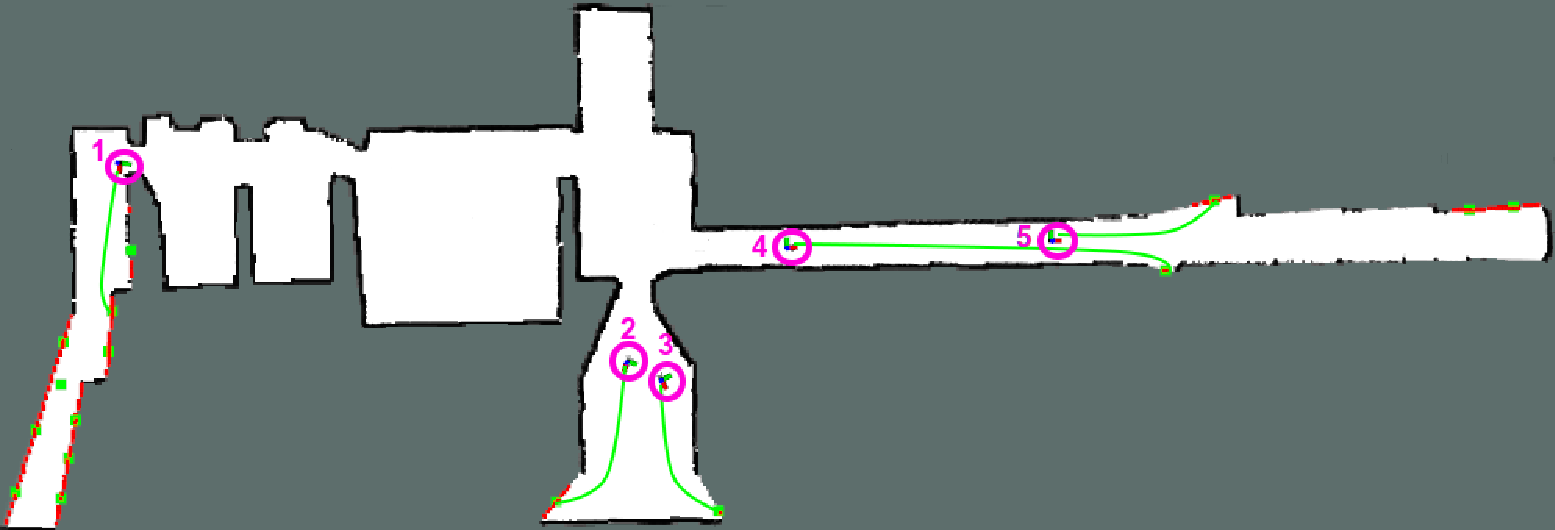
\includegraphics[width=0.85\textwidth]{figures/siminprogress1}
	%\caption{Autonomous exploration using multi-robot system. Mobile robots focused on different target points according to an exploration strategy.}
	\end{figure}
\end{frame}

\begin{frame}
	\frametitle{Multi-robot exploration}
	\begin{itemize}
		\item[-] \textbf{ADVANTAGES:}
		\begin{itemize}
			\item[-] Robustness %(due to redundancy)
			\item[-] Efficiency %(a robot team can accomplish a predefined task much quicker than a single robot can\footcite{Dias2000})
			\item[-] Sensor fusion\footcite{Wurm2008} %(can compensate sensor uncertainty)
%			\item[-] Free from single-point failure (if system is decentralized)
			\item[-] Larger range of task domains\footcite{Dias2006}
		\end{itemize}
		\item[-] \textbf{DISADVANTAGES:}
		\begin{itemize}
			\item[-] High communication requirement% in general
			\item[-] If greedy assignment methods are used, convergence to a suboptimal goal is possible
		\end{itemize} 
	\end{itemize}
\end{frame}

\begin{frame}
	\frametitle{Problem formulation}
%		\item[-] The goal of an exploration strategy consists in increasing robots knowledge of the environment by selecting appropriate control actions with the objective to minimize the size of the unexplored area. 		
	\begin{columns}
		\begin{column}{0.5\textwidth}
			\begin{itemize}
				\item[-] Given a team of $n$ robots ($r_{1}$,...,$r_{n}$), the goal of the exploration	strategy is twofold:
				\begin{itemize}
					\item[1)] \textbf{Compute effective targets} ($w_{1}$,...,$w_{m}$) 
					\item[2)] \textbf{Coordination strategy:} which robot to which target 
				\end{itemize}			
			\end{itemize}
		\end{column}
		\begin{column}{0.5\textwidth}  %%<--- here
			\begin{center}
				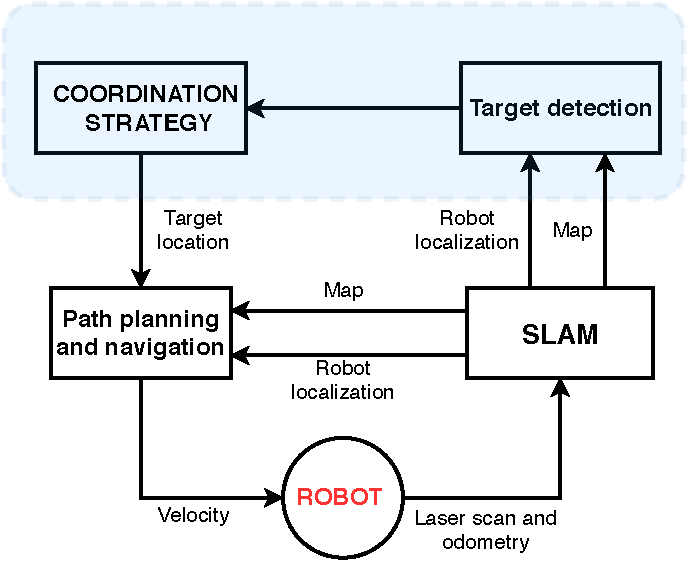
\includegraphics[width=1\textwidth]{figures/strategy_all}
				\label{fig:gauss}
			\end{center}
		\end{column}
	\end{columns}	
\end{frame}

%\begin{frame}
%	\frametitle{Problem formulation (2)}
%	\begin{figure}
%		\centering
%		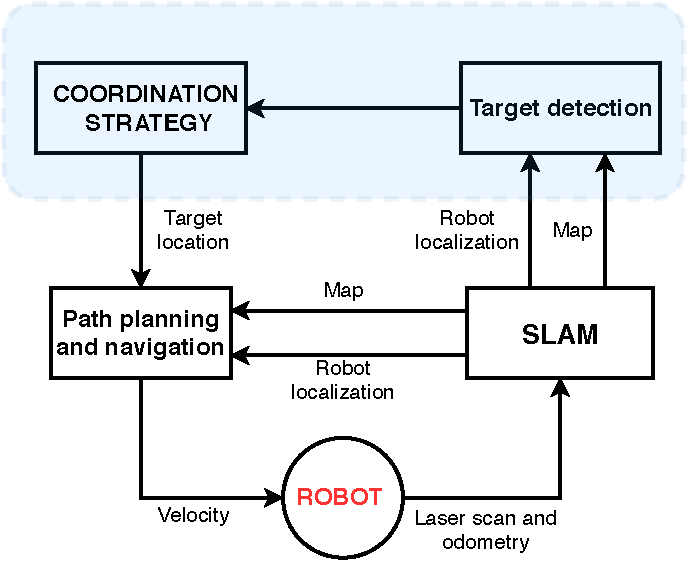
\includegraphics[width=0.6\textwidth]{figures/strategy_all}
%		\caption{The overall frontier exploration and mapping process for a single robot that can be easy extended to multi-robot system.}
%	\end{figure}
%\end{frame}

\begin{frame}
	\frametitle{Computing effective targets - frontier detection (1)}
	\begin{itemize}
		\item[-] \textbf{Occupancy grid map} - discretizes the environment into a grid of map cells\footcite{Moravec}
		\item[-] \textbf{Free, occupied or unknown}
		\item[-] \textbf{Frontier} introduced by Yamauchi\footcite{Yamauchi1997} 				
	\end{itemize}
	\begin{figure}
		\centering
		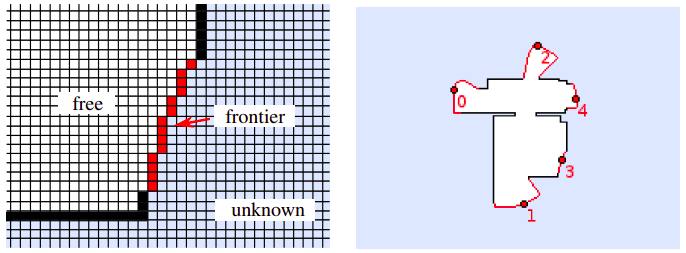
\includegraphics[width=0.75\textwidth]{figures/environment1}
		%\caption{2D occupancy grid map: unknown cells are shown light blue, free cells are depicted in white and occupied cells (obstacles) in black. Left: Frontier cells (red) are determined at the boundary between free and unknown map cells. Right: Five exploration targets, visualized as red circles, are generated at frontiers (Source\footcite{Wurm2012})}
	\end{figure}
\end{frame}

\begin{frame}
	\frametitle{Computing effective targets - frontier detection (2)\footcite{Umari2017}$\,$\footcite{Orsulic2019}}
		\begin{columns}
				\begin{column}{0.5\textwidth}\centering
					{\bf{RRT frontier detection}}\\ 
					\vspace{0.2cm}
					\begin{center}
						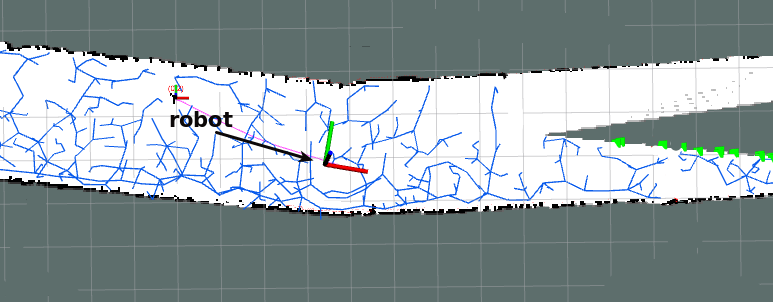
\includegraphics[height=2.3cm]{figures/rrt2}
						%\caption{Industrial Manipulator KUKA KR30}
						\label{fig:cent}
					\end{center}
					\vspace{0.1cm}
					%\begin{itemize}
						%\item[-] RRT frontier detection%\footcite{Umari2017}
					%\end{itemize}
				\end{column}
				\begin{column}{0.5\textwidth}\centering
					{\bf{Efficient dense frontier detection}}\\ 
					\vspace{0.2cm}
					\begin{center}
						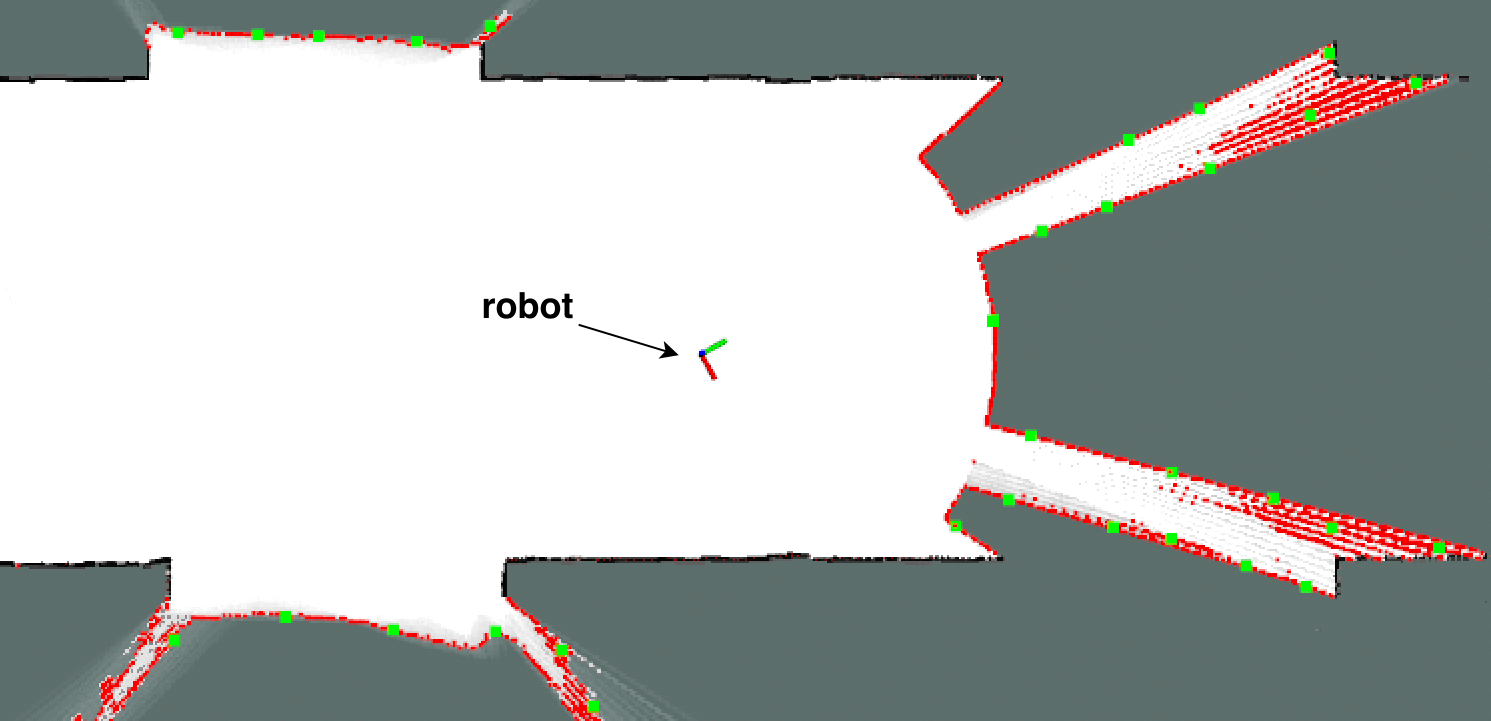
\includegraphics[height=2.3cm]{figures/carto1}
						%  \caption{Collaborative Manipulator KUKA IIWA}
						\label{fig:decent}
					\end{center}
				\end{column}
			\end{columns}
\end{frame}
		
\begin{frame}
	\frametitle{Coordination algorithms}
		\begin{figure}
			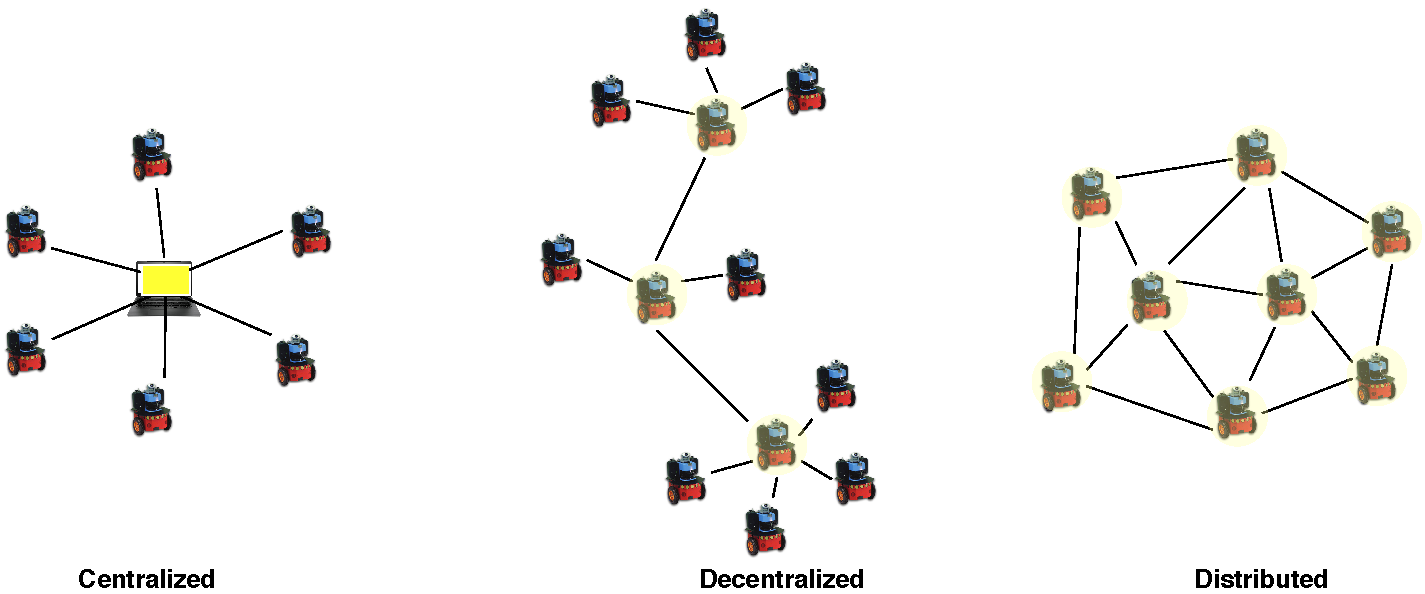
\includegraphics[width=1\textwidth]{figures/robots}
			%\caption{Industrial Manipulator KUKA KR30}
			\label{fig:cent}
		\end{figure}
%	\begin{columns}
%		\begin{column}{0.5\textwidth}\centering
%			{\bf{Centralized}}\\ 
%			\vspace{0.1cm}
%			\begin{center}
%				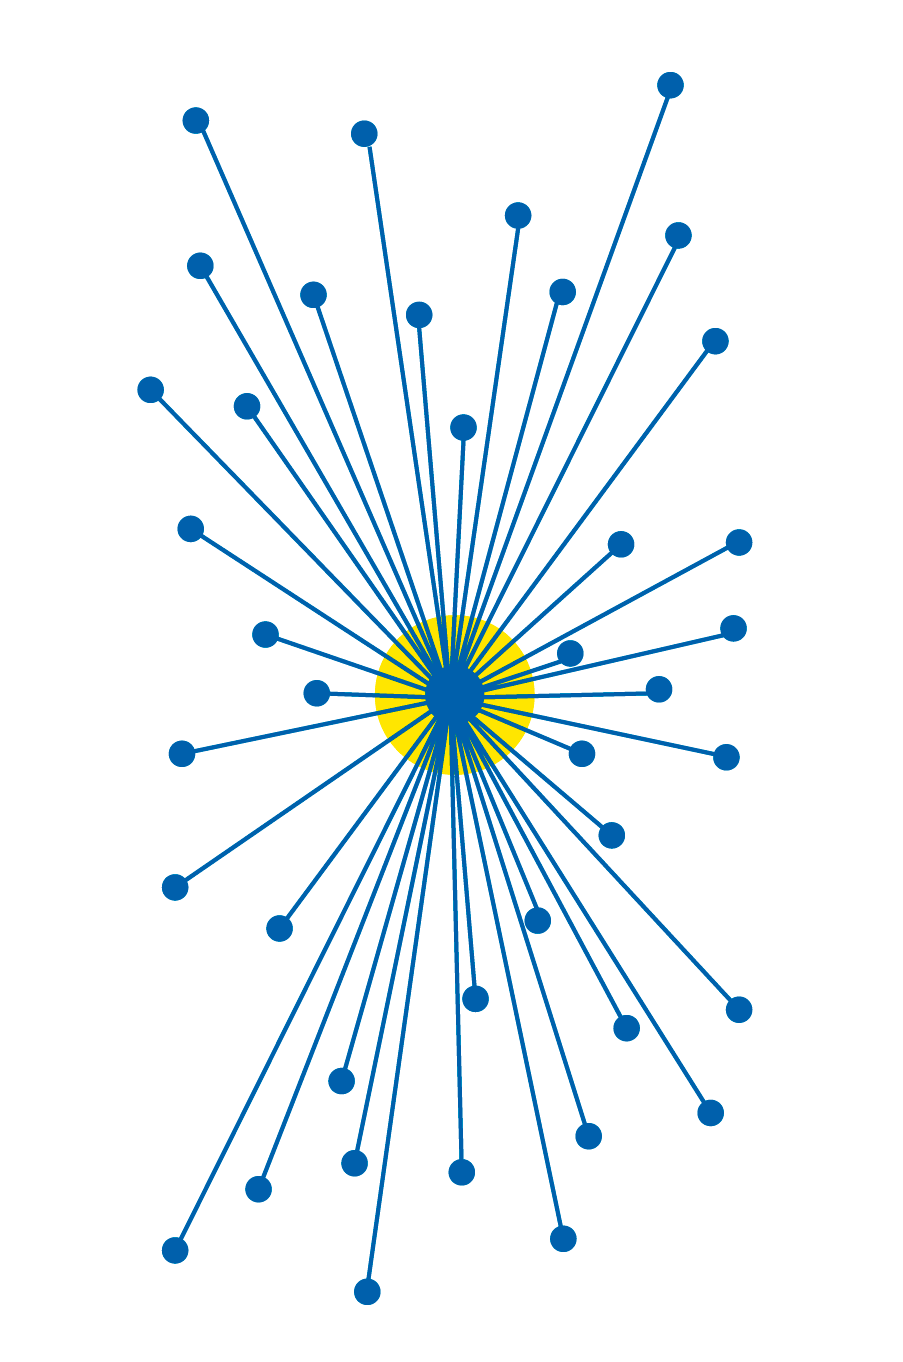
\includegraphics[height=3cm]{figures/cent}
%				%\caption{Industrial Manipulator KUKA KR30}
%				\label{fig:cent}
%			\end{center}
%			\vspace{0.01cm}
%			\begin{itemize}
%				\item[-] Single central \textit{leader}
%				\item[-] Communication limits and robustness issues 
%				\item[-] Optimal plans can be found
%			\end{itemize}
%		\end{column}
%		\begin{column}{0.5\textwidth}\centering{\bf{Decentralized }}\\
%			\vspace{0.1cm}
%			\begin{center}
%				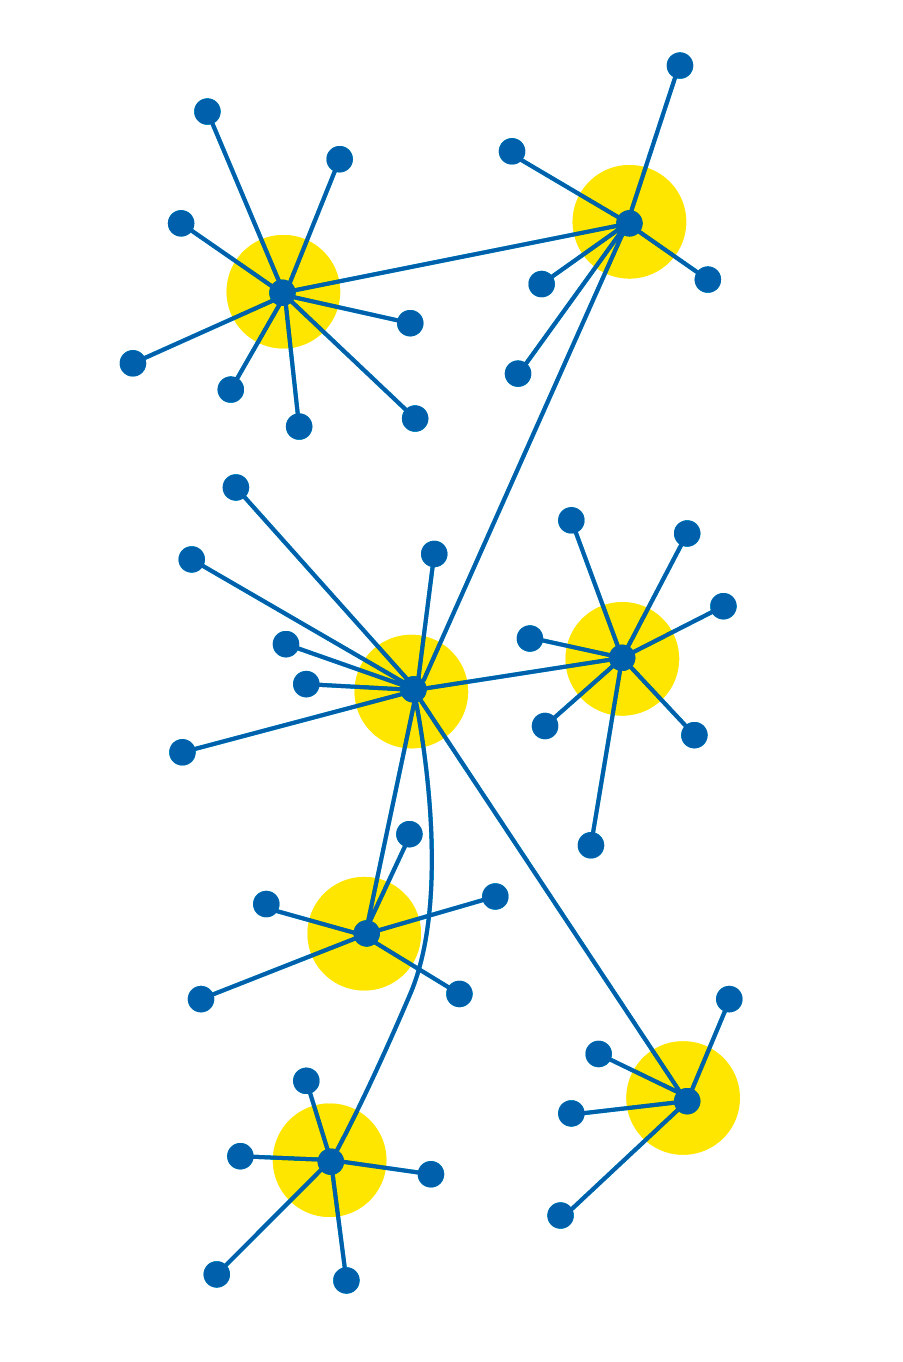
\includegraphics[height=3cm]{figures/decent}
%				%  \caption{Collaborative Manipulator KUKA IIWA}
%				\label{fig:decent}
%			\end{center}
%			\vspace{0.01cm}
%			\begin{itemize}
%				\item[-] Robots are completely (or at least partially) independent
%				\item[-] Better reliability, flexibility, adaptability and robustness
%			\end{itemize}
%		\end{column}
%	\end{columns}
	
\end{frame}


%\begin{frame}
%	\frametitle{Motivation}
%	\begin{columns}
%		\begin{column}{0.5\textwidth}
%			\begin{itemize}
%				\item Industrial scenario : Delicate sanding of complex shape surfaces in aerial industry 
%				\item Robot sanding using Kuka KR30 equipped with ACF (Active Contact Flange)
%				\item Goal: Create robotic sanding system capable to control contact force in 6 DOF
%			\end{itemize}
%		\end{column}
%		\begin{column}{0.5\textwidth}  %%<--- here
%			\begin{center}
%				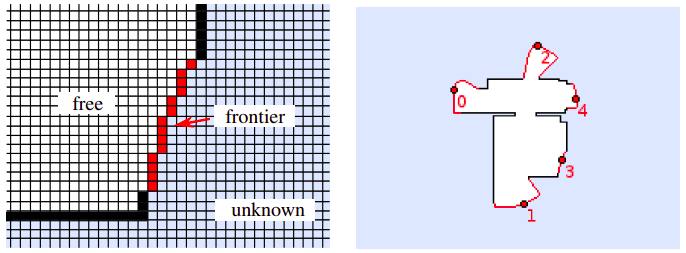
\includegraphics[width=1\textwidth]{figures/environment1}
%				\label{fig:enikon_kuka}
%			\end{center}
%		\end{column}
%	\end{columns}
%\end{frame}
%\begin{frame}
%     \frametitle{Effective Robotic GriNDing of Surface Areas through HORSE framework (ENDORSE)}
%     \begin{columns}
%        \begin{column}{0.3\textwidth}
%            \begin{itemize}
%                 \item \textbf{Compliant control algorithm}
%                 \item Human oriented machine interface
%                 \item Safety of human
%                 \item Automated quality inspection system
%            \end{itemize}
%        \end{column}
%        \begin{column}{0.7\textwidth}  %%<--- here
%            \begin{center}
%             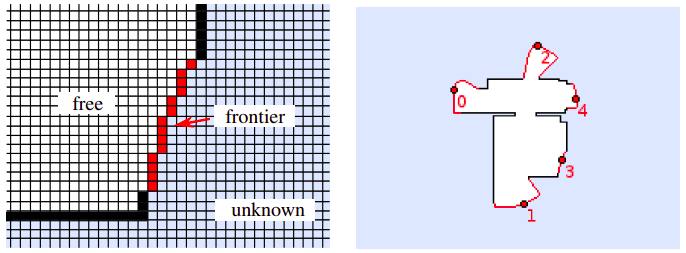
\includegraphics[width=1\textwidth]{figures/environment1}
%            %  \caption{ENDORSE setup}
%             \label{fig:enikon_kuka}
%             \end{center}
%        \end{column}
%    \end{columns}
%\end{frame}

\section{2D coordination algorithms}

\subsection{Nearest frontier approach}
\begin{frame}
     \frametitle{Nearest frontier approach}
     \begin{itemize}
     	\item[-] Choose the nearest frontier region to explore
%     	\item[-] Yamauchi's technique consists in selecting the shortest path to the nearest frontier. 
     	\item[-] The target cell:
     	\begin{equation}
     	t_{NF} = \argmin_{a \in F} L(a)
     	\label{equation:t-nf}
     	\end{equation}	
     	\item[-] “Given what you know about the world, where should you move to gain as much new	information as possible?”\footcite{Yamauchi1998} 
     	\item[-] Extension to multiple robots
     \end{itemize}
     
\end{frame}

\subsection{Cost-utility approach}
\begin{frame}
	\frametitle{Cost-utility approach}
	\begin{itemize}
		\item[-] Next-Best-View\footcite{GonzlezBaos2002} 
		\item[-] The benefit $B_{CU}(a)$ to reach a candidate cell $a$:
		\begin{equation}
		B_{CU}(a) = U(a) - \lambda_{CU}C(a)
		\label{equation:cost-utility}
		\end{equation}
%		\begin{equation}
%		U(a) = \frac{U_{nex}(a, R_{s})}{\pi R_{s}^{2}}
%		\end{equation}
%		\begin{equation}
%		C(a) = \frac{L(a)}{max_{b \in F}L(b)}
%		\end{equation}
		\item[-] The target cell $t_{CU}$:
		\begin{equation}
		t_{CU} = \argmax_{a \in F} B_{CU}(a)
		\end{equation}
		\item[-] Coordination by reducing the utility of a frontier point\footcite{Burgard2000}
		\item[-] Optimized using the Hungarian method\footcite{Burgard2005}
	\end{itemize}
	
\end{frame}

\subsection{Market-based approach}
\begin{frame}
	\frametitle{Market-based approach}
%	\begin{figure}
%		\centering
%		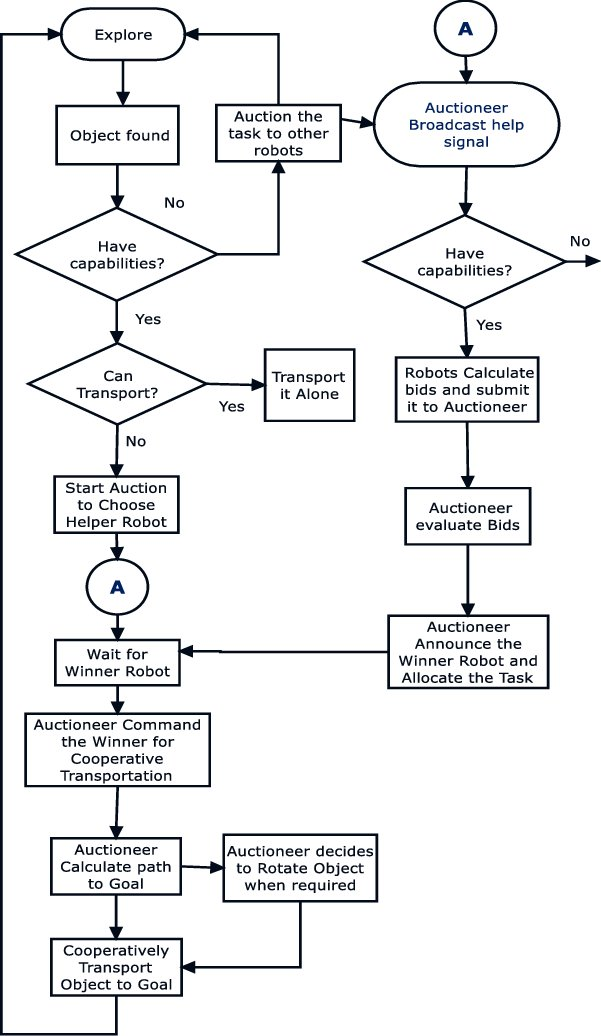
\includegraphics[height=6cm, width=5cm]{figures/auction}
%%		\caption{Auction}
%	\end{figure}
	\begin{itemize}
		\item[-] Introduced by Zlot\footcite{Zlot2002}
		\item[-] Robots as \textbf{sellers} and \textbf{buyers}
%		\item[-] %After reaching a current goal point,
		\item[-] A robot initiates an \textbf{auction}
		\begin{equation}
			B_{i} = P_{r} + \alpha(v_{i} - P_{r})
		\end{equation}
%		Next, the robot tries
%		to sell each of its tasks to all robots with which it is currently able to communicate, via an auction. The other
%		robots each submit bids, which encapsulate their cost
%		and revenue calculations. The robot offering the task
%		(the auctioneer) waits until all robots have bid (up to a
%		specified amount of time). If any robot bids more than
%		the minimum price set by the auctioneer, the highest
%		bidder is awarded the task in exchange for the price of
%		the bid. Once all of a robot’s auctions close (all goals
%		on the robot’s tour have been sequentially offered),
%		that robot begins its tour by navigating towards its
		\item[-] The highest bidder is awarded 		
%		\item[-] For each point in auction, each robot makes a bid with its current profit aiming to minimize own travel distance and maximize new area information
%		not	dependent the central agent
		\item[-] Market model with limited communication range \footcite{Sheng2006} $\,$ \footcite{Michael2008}
		
%		W. Sheng, Q. Yang,
%		S. Ci and N. Xi [7] are proposed another, frontier based, distributed bidding model for
%		coordination of multiple robots. Besides, they consider the limited communication
%		environment in two ways. Firstly, they guided robots to stay close to each other by
%		considering the distances between robots in the coordination algorithm. Additionally,
%		they developed a new coding mechanism for map representation. New coding mechanism
%		reduced the exchanged data volume.
%Michael et al. [35] proposed a marked-based coordi-nation protocol where robots are able to bid for taskassignment with the assumption that every robot hasknowledge of the maximum number of robots that anygiven task can accommodate. Each auction is performedamong neighboring groups of robots and requires onlylocal communication.
%		
		\end{itemize}
	
\end{frame}

\subsection{Distributed approach}
\begin{frame}
	\frametitle{Distributed approach}
	\begin{itemize}
		\item[-] A team of $n$ mobile robots  \(\text{$\mathcal {R}$}\) = $ \{ 1, 2,..., N\}$
		\item[-] Every robot $i$ gets the list of frontier points  \(\text{$\mathcal {Y}$}\) = $ \{ 1, 2,..., M\}$
	\end{itemize}
%	The exploration is performed by, where the mobile robots do not have prior knowledge about the environment, i.e., the position of the boundaries and obstacles.  
	
	\begin{figure}
		\centering
		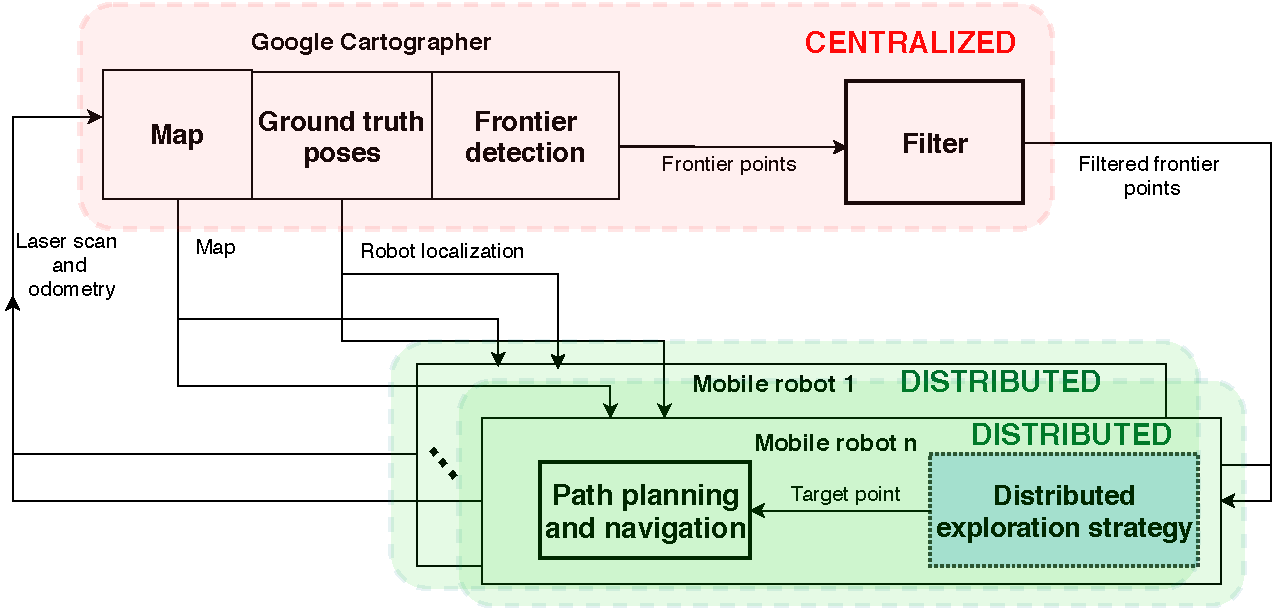
\includegraphics[width=0.9\textwidth]{figures/diagram_exploration}
	\end{figure}
\end{frame}

\begin{frame}
	\frametitle{Distributed exploration strategy}
		\begin{columns}
			\begin{column}{0.5\textwidth}
				\begin{itemize}
					\item[-] Information exchanged: robot positions and current robot target point. 
					\item[-]  \textit{Weight function}: 
					\begin{equation}
					{W}_{ij}= {C_{ij}} - {U_{j}} + {F_{ij}}.
					\label{weight}
					\end{equation}
					\item[-] \textbf{Event-based} target point assignment process  
				\end{itemize}
			\end{column}
			\begin{column}{0.5\textwidth}  %%<--- here
				\begin{center}
					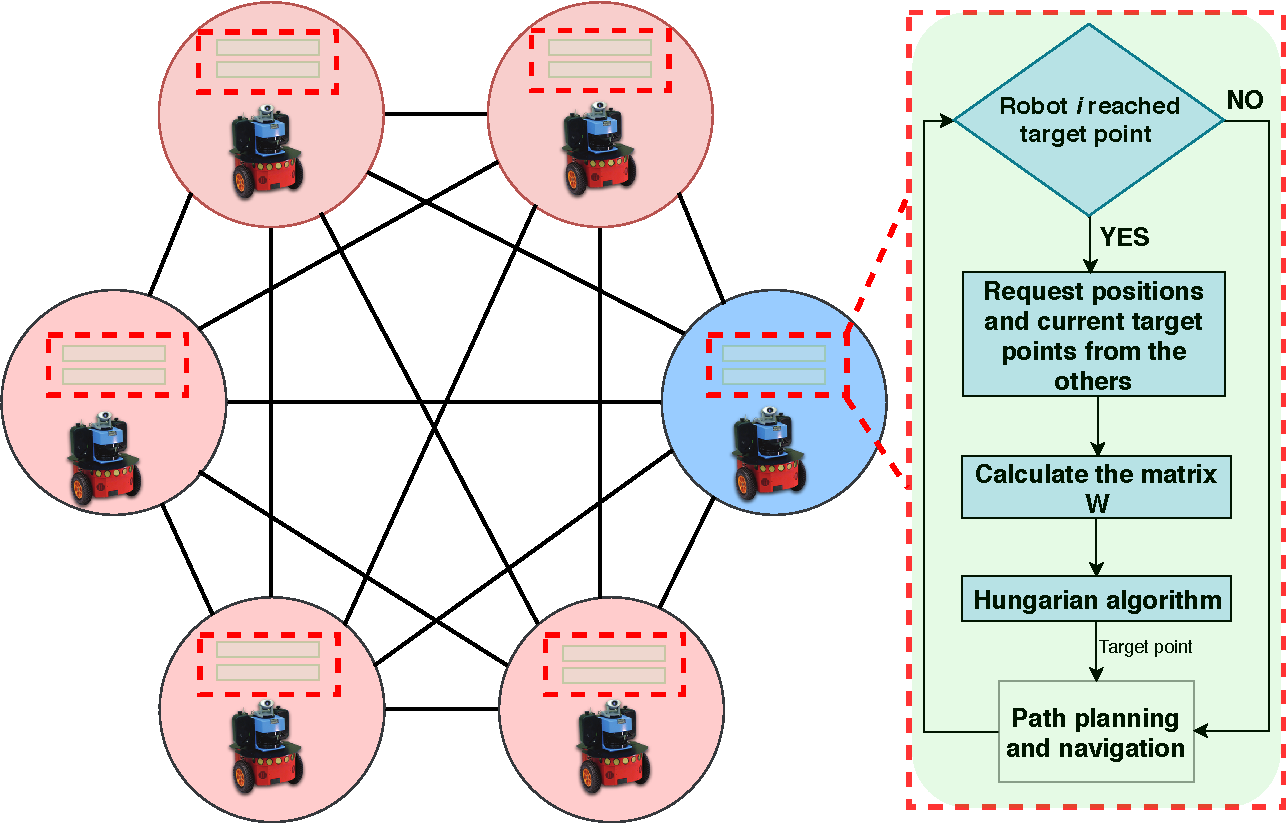
\includegraphics[width=1\textwidth]{figures/struktura_vol3}
					\label{fig:gauss}
				\end{center}
			\end{column}
		\end{columns}	
\end{frame}

\begin{frame}
	\frametitle{Distributed exploration strategy - simulation setup (1)}
	\begin{itemize}
		\item[-] Stage 2D simulator
		\item[-] Belgioioso Castle\footcite{fr_dataset} $\approx$ 225$m^{2}$
		\item[-] 2, 3 and 5 Pioneer P3-DX mobile robots
		\item[-] Average of 10 runs 
		\item[-] Compared with the Burgard's coordinated strategy
		\item[-] \textit{Coverage Ratio (CR)}:  \( \frac{\text{explored cells} \cdot 100}{\text{accessible cells}} \)
%The comparison of the coordinated and our decentralized strategy is shown using the \textit{Coverage Ratio (CR)} indicator which shows the percentage of the accessible terrain covered by the mobile robot team. It is calculated as:  \( \frac{\text{explored cells} \cdot 100}{\text{accessible cells}} \), 
	\end{itemize}
%	Simulations  were  carried  out  using  the  Stage  2D  simulator(Vaughan et al. (2012)), which simulates robot movement andlidar perception inside a loaded environment map. The ROSNavigation stack is used to control and direct the mobile robotstowards exploration goals.The scenario used in the simulation is the Belgioioso Castle,available  in  Haehnel  (2014)  and  shown  in  Fig.  5.  It  is  achallenging and a typical office-like scenario with a free spacearea of approximately 225m2. For the simulation, we use amodel of Pioneer P3-DX with maximum speed of 1.3 m/s, laserrange 20 m and 360◦laser scan window.The  algorithms  were  tested  with  teams  of  two,  three  andfive mobile robots
	\begin{figure}
		\centering
		
\includegraphics[width=0.6\textwidth]{figures/map}
	\end{figure}
\end{frame}

\begin{frame}
	\frametitle{Distributed exploration strategy - simulation setup (2)}
		\centering
		\href{presentation_video.mp4}{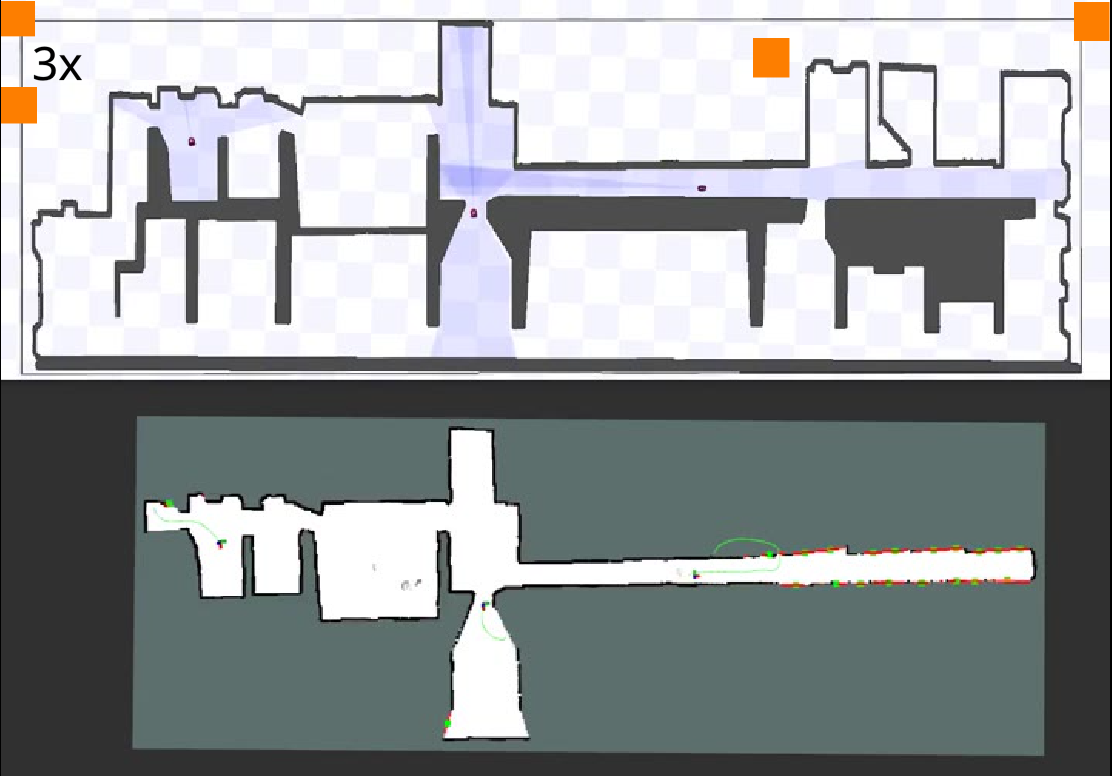
\includegraphics[width=0.8\textwidth]{figures/title_screen.png}}
\end{frame}

\begin{frame}
	\frametitle{Distributed exploration strategy - simulation results}
	\begin{figure}
		\centering
		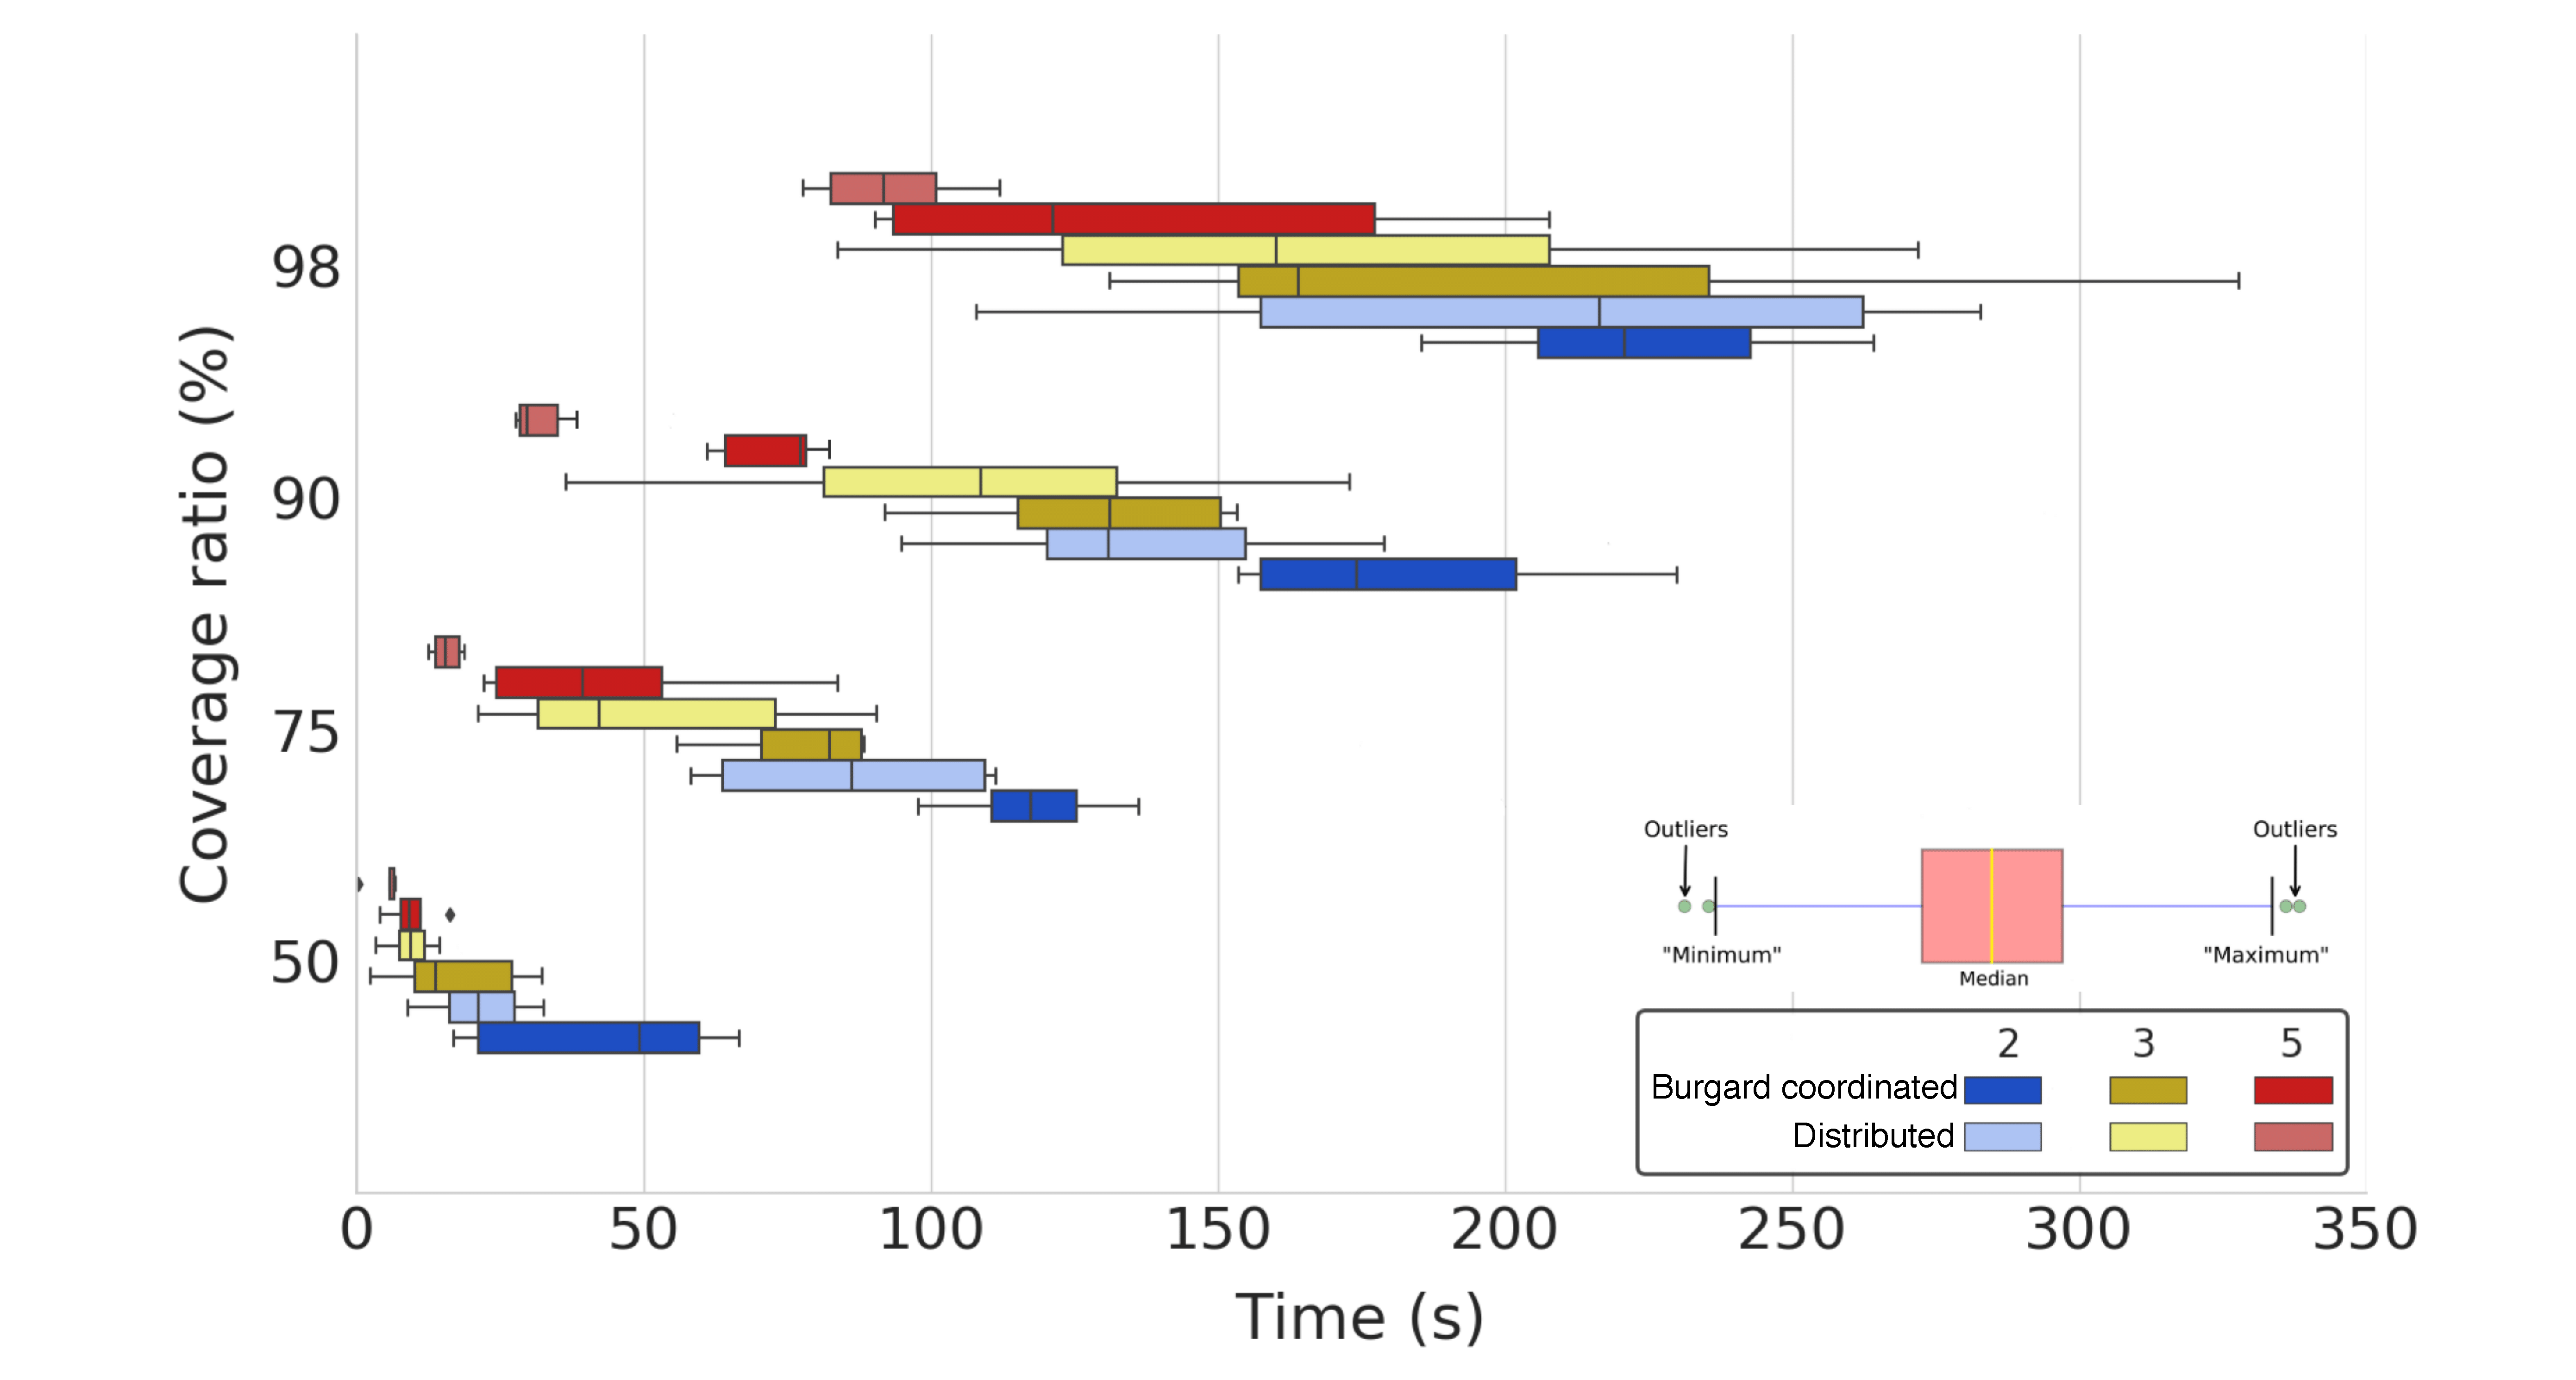
\includegraphics[width=1\textwidth]{figures/results_final}
	\end{figure}
\end{frame}



\section{3D coordination algorithms}

\begin{frame}
	\frametitle{Motivation}
	\centering
	\href{mbzirc_video.mp4}{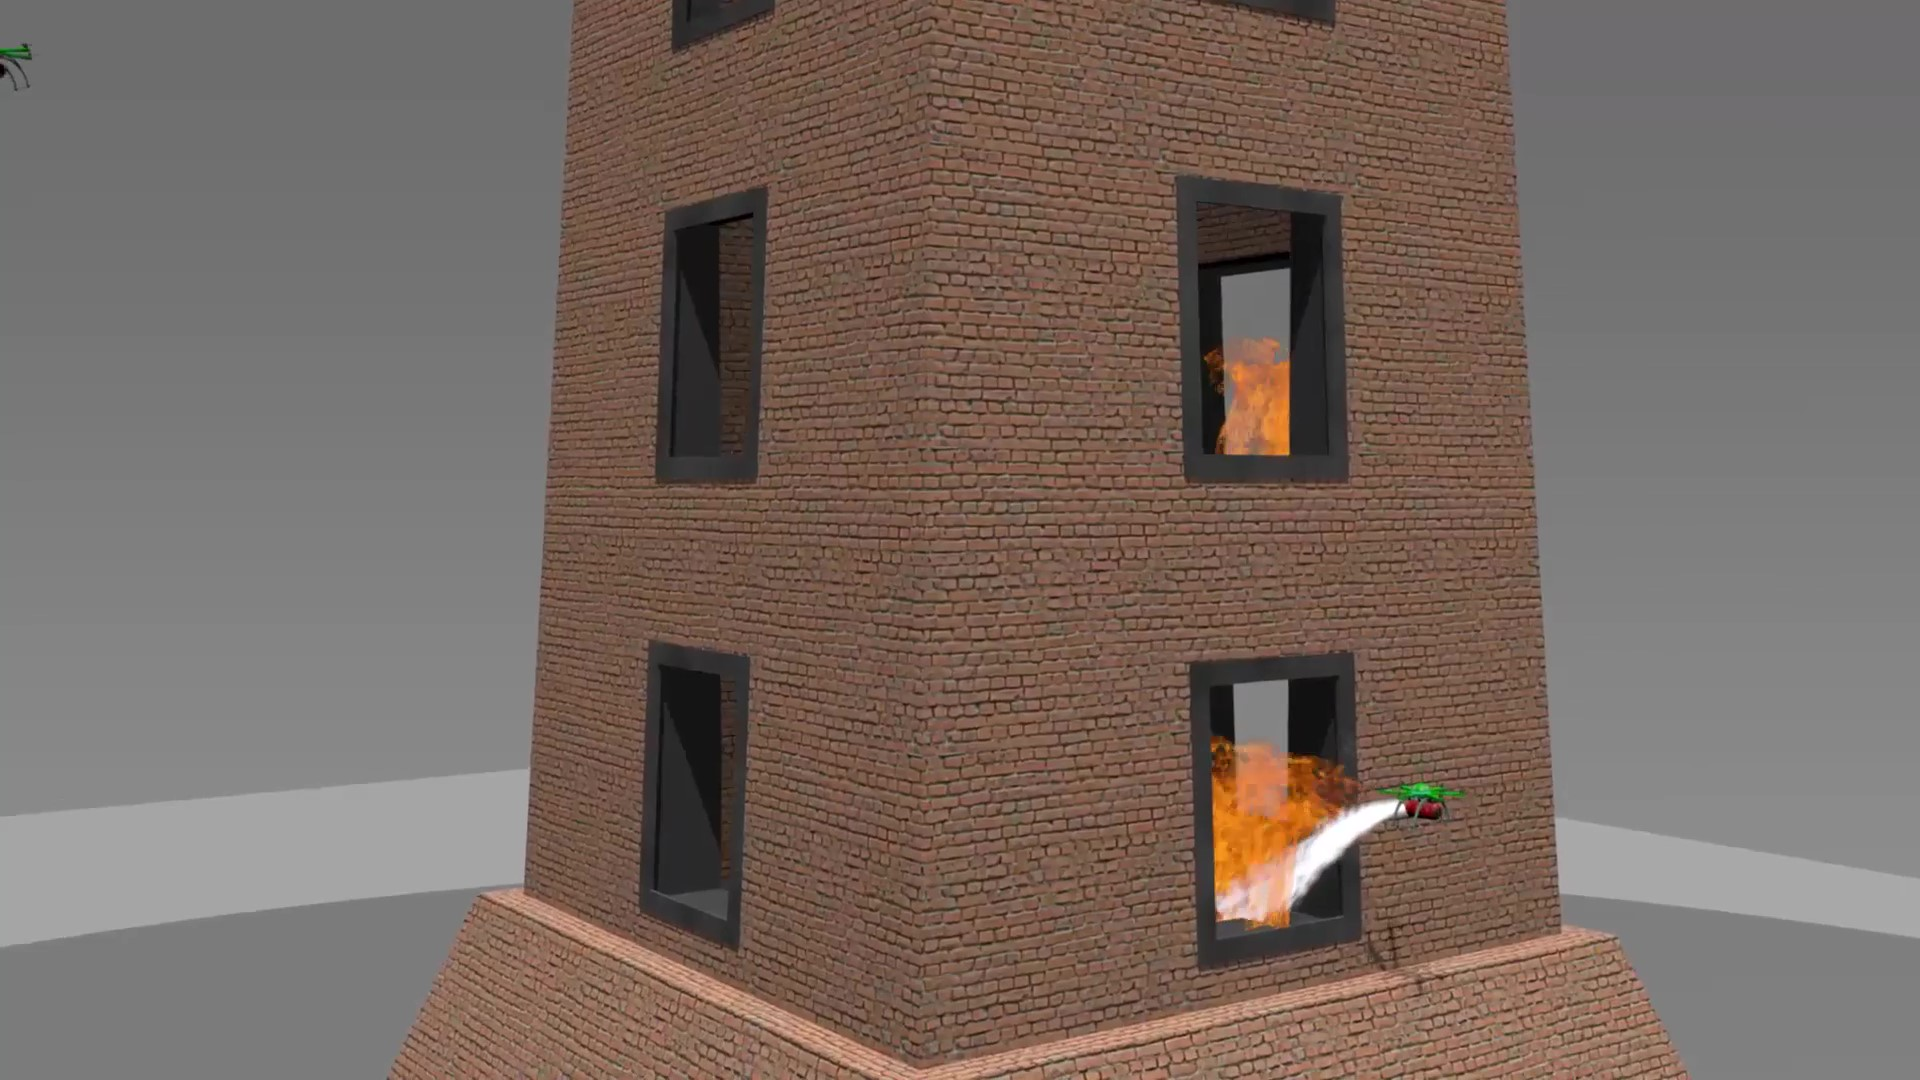
\includegraphics[width=0.8\textwidth]{figures/mbzirc_screen.jpg}}
	
\end{frame}

\subsection{Extension of 2D exploration solutions to 3D solution}
\begin{frame}
     \frametitle{Extension of 2D exploration solutions to 3D}
     \begin{itemize}
     	\item[-] Reducing the dimension of the navigation space of robots\footcite{Bachrach2009}$\,$\footcite{Surmann2003}
     	\begin{itemize}
     		\item[-] 2.5D elevation maps 
     		%\item[-] Resulting model would probably contain unexplored areas
     	\end{itemize}	
     	\item[-] A complete 3D exploration is proposed in 2013 by Dornhege\footcite{Dornhege2013}
%     	algorithm was tested on a 5-DOF manipulator with a workspace radius of one
%     	meter
     	 %(i.e., an extension of Next-Best-View method to 3D)
     	 	\begin{itemize}
     			\item[-] Can be applied only in small areas (\textbf{computational effort})
     	 	\end{itemize}
      	\item[-] Combination of 2D and 3D exploration strategies\footcite{Maurovic2014}
      	%based on next-best-view method and room detection (Maurovic\footcite{Maurovic2014})
      	\begin{itemize}
      		\item[-] The robot switches to 3D exploration while a room is detected
      		\item[-] Local maps of rooms
      		% are used to overcome the problem of computational effort and memory consumption
      	\end{itemize}		
     \end{itemize}   
\end{frame}

\subsection{3D exploration - single robot}
\begin{frame}
	\frametitle{3D exploration - single robot}
	\begin{itemize}
		\item[-] Formalized extension of the \textbf{frontier-based exploration}\footcite{ShadeNewman2011}
		\item[-] Next-best-view approach for 3D exploration\footcite{Bircher2016}
		
%		Shade and Newmann formalize, in [15], the 3D extension of
		%the frontier-based exploration. In particular, 3D frontiers are integrated with a
		%vector field approach to achieve 3D exploration with a stereo camera. 
		%3D requires highmemory and computational consumptions
		\item[-] Extraction of 3D frontiers from the OctoMap\footcite{Zhu2015}
%		\begin{itemize}
%			\item[-] Extract the 3D	frontiers from the OctoMap
%		\end{itemize}
		\item[-] 3D exploration based on surface frontier voxels \footcite{Senarathne2016} 
		\begin{figure}
			\centering
			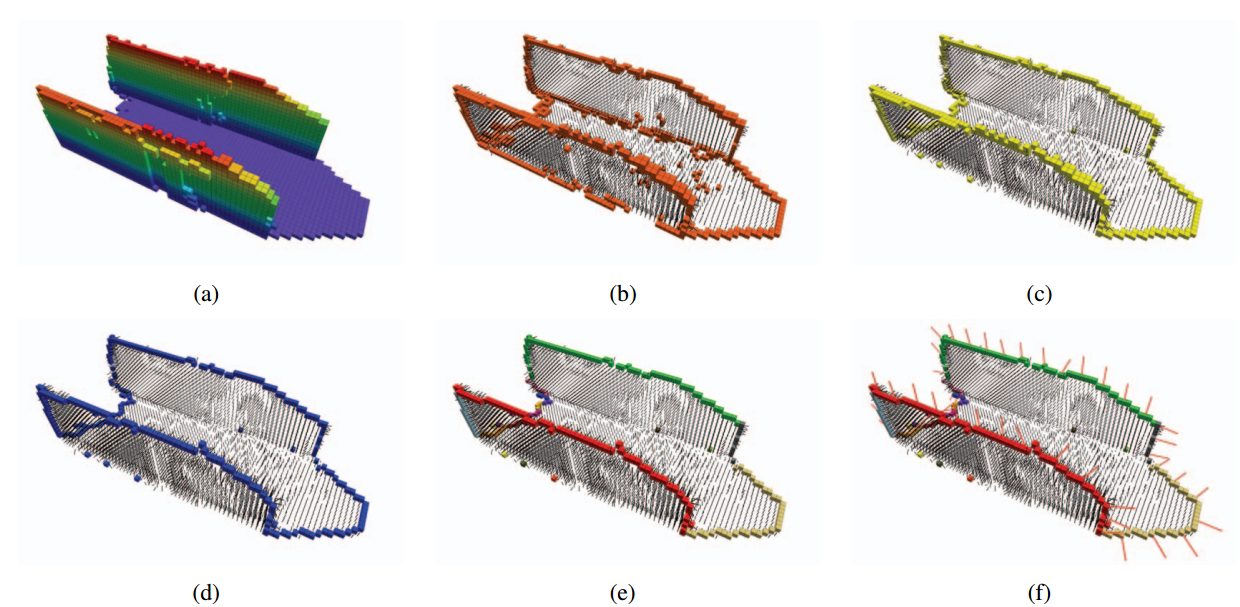
\includegraphics[width=0.5\textwidth]{figures/senarathne}
		\end{figure}
		
%presented an alternative approach to 3D exploration based on surface frontier voxels. The strategy focuses on seeking the expansion of mapped surfaces, instead of reducing unmapped voxels.
		
	\end{itemize}	
\end{frame}
%Next-best-view approach in the process of building 3D model of a real object used without any a priori information about the environment was described in \cite{VasquezGomez2014}. The algorithm determines each view to reconstruct an arbitrary object. Furthermore, authors proposed a method to deal with the uncertainty in sensor positioning.
%Next-best-view approach for 3D exploration was presented by Bircher et. al. \cite{Bircher2016}. Authors presented a novel path planning algorithm for the autonomous exploration of an unknown area. The proposed planner finds the best branch in an online computed tree. The quality of the branch is determined by the amount of unmapped space that can be explored. The planner is capable of running online, onboard a robot with limited resources.
%\begin{frame}
%     \frametitle{Extension of 2D exploration solutions to 3D (3)}
%		\begin{itemize}
%			\item[-]  for indoor environment
%			\item[-] Frontiers are searched just on a subset of nodes, the changed cells\footcite{Keidar2012}
%			\item[-] Method suffers from local minima
%			\item[-] The application in uncluttered environments results in few uninformative frontiers
%		\end{itemize}
%\end{frame}
\subsection{3D exploration - multi-robot}
\begin{frame}
	\frametitle{3D exploration - multi-robot}
	\begin{itemize}
		\item[-] An entropy-based measure of information utility\footcite{Rocha2005}
		% to define a cooperation strategy for sharing useful information
		\item[-] Minimization of accumulative data errors during the exploration\footcite{Vutetakis2019}
		\item[-] An information potential field based method\footcite{Wang2019} 
		\begin{itemize}
			\item[-] Reduce path cost and map entropy (an uncertainty of the map)
		\end{itemize} 
		\begin{figure}
			\centering
			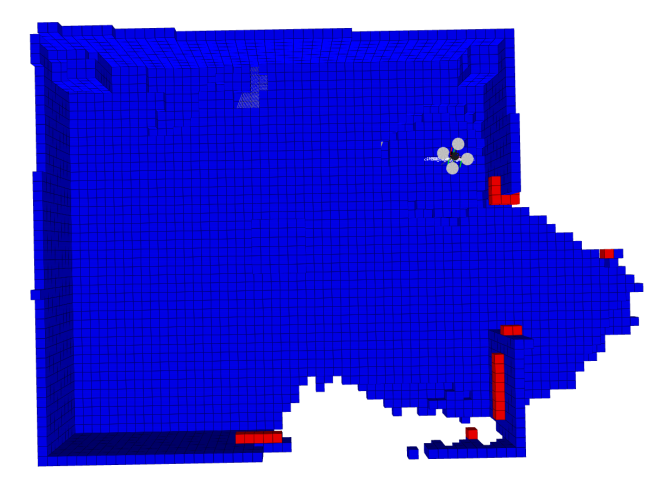
\includegraphics[height=2cm]{figures/frontier_extraction}
		\end{figure}
%Vutetakis in \cite{Vutetakis2019} proposed a novel strategy for inspecting critical infrastructure autonomously using Micro Aerial Vehicles (MAVs). In order to facilitate autonomous inspection capabilities, this strategy addresses the problem of autonomous MAVs exploration and coverage of an unknown structure to acquire the spatial information necessary for the development of a high-fidelity 3D model of the structure. Key to this problem is to not only cover the entire structure, but also to minimize accumulative data errors during the exploration through direct planning of loop closures. 

%Rocha et al. \cite{Rocha2005} dealt with 3D mapping by multiple robots using cubic cells for information storage. Authors presented a technique which is used for frontier-based exploration. At the beginning of the exploration an initial map is given to the robot, the robots update old map by new set of information obtained through sensing and share their useful information with other robots. The process is repeated until the whole area is explored and mapped.

%The 3D exploration problem using aerial vehicles within limited flight endurance was addressed by Wang et al. \cite{Wang2019}. Authors proposed an information potential field based method considering both the traveled cost and information-gain. The next-best-view point is chosen based on a multi-objective function which considers information of several candidate regions and the traveled path cost. The selected goal
%attracts the robot while known obstacles form the repulsive
%force repel the robot.
				
	\end{itemize}	
\end{frame}

\subsection{Firefighting mission}
\begin{frame}
	\frametitle{Firefighting mission - frontier exploration (1)}
	\begin{columns}
		\begin{column}{0.5\textwidth}\centering
			\begin{center}
				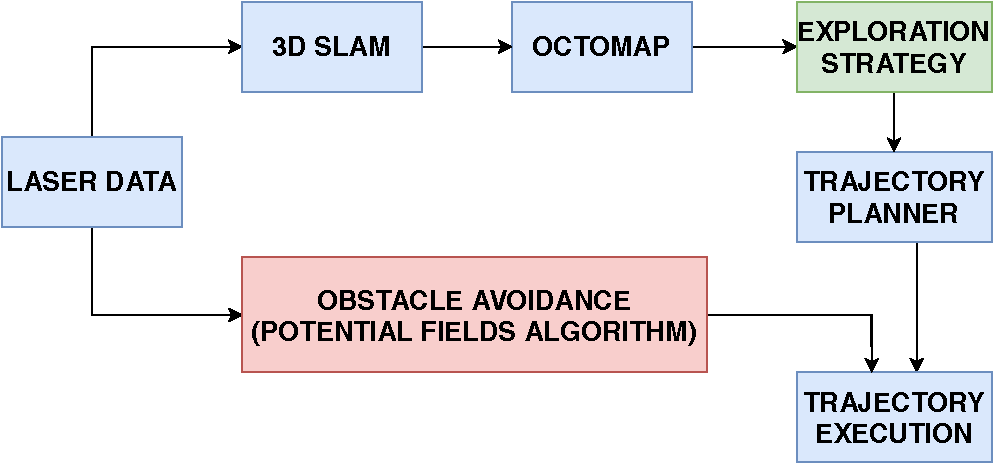
\includegraphics[height=3cm]{figures/3D_strategy}
				\label{fig:forest_uav}
			\end{center}
			%			\vspace{0.1cm}
			%			\begin{itemize}
			%				\item Stiff position-controlled
			%				\item Payload: 10-300 kg
			%				\item High speed, high accuracy
			%			\end{itemize}
		\end{column}
		\begin{column}{0.4\textwidth}\centering
		\begin{itemize}
			\item[-] GPS building location
			\item[-] Google Cartographer SLAM
		\end{itemize}
			%			\vspace{0.1cm}
			%			\begin{itemize}
			%				\item Joint torque-controlled
			%				\item Payload: up to 15 kg
			%				\item Environment sensing
			%			\end{itemize}
		\end{column}
	\end{columns}
\end{frame}

\begin{frame}
	\frametitle{Firefighting mission - frontier exploration (2)}
	\begin{figure}
		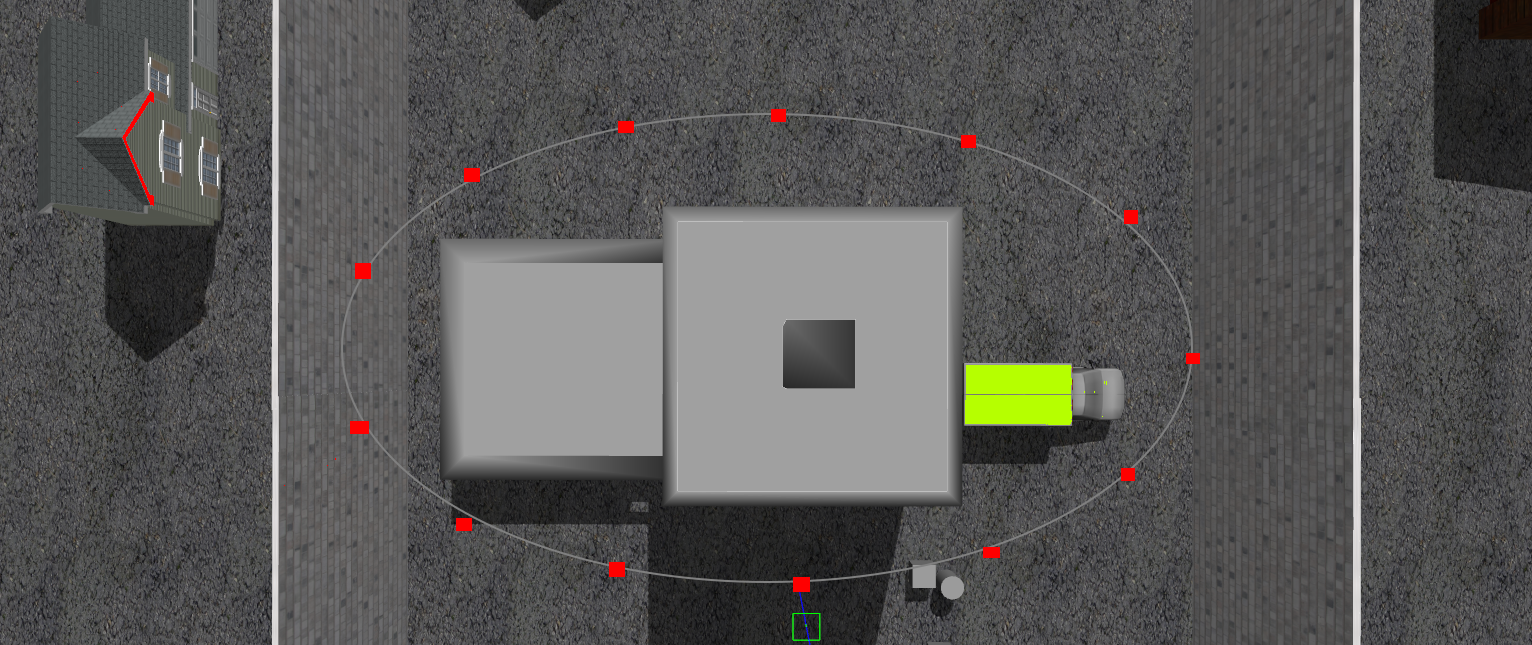
\includegraphics[height=3cm]{figures/building}
	\end{figure}
	\begin{figure}
	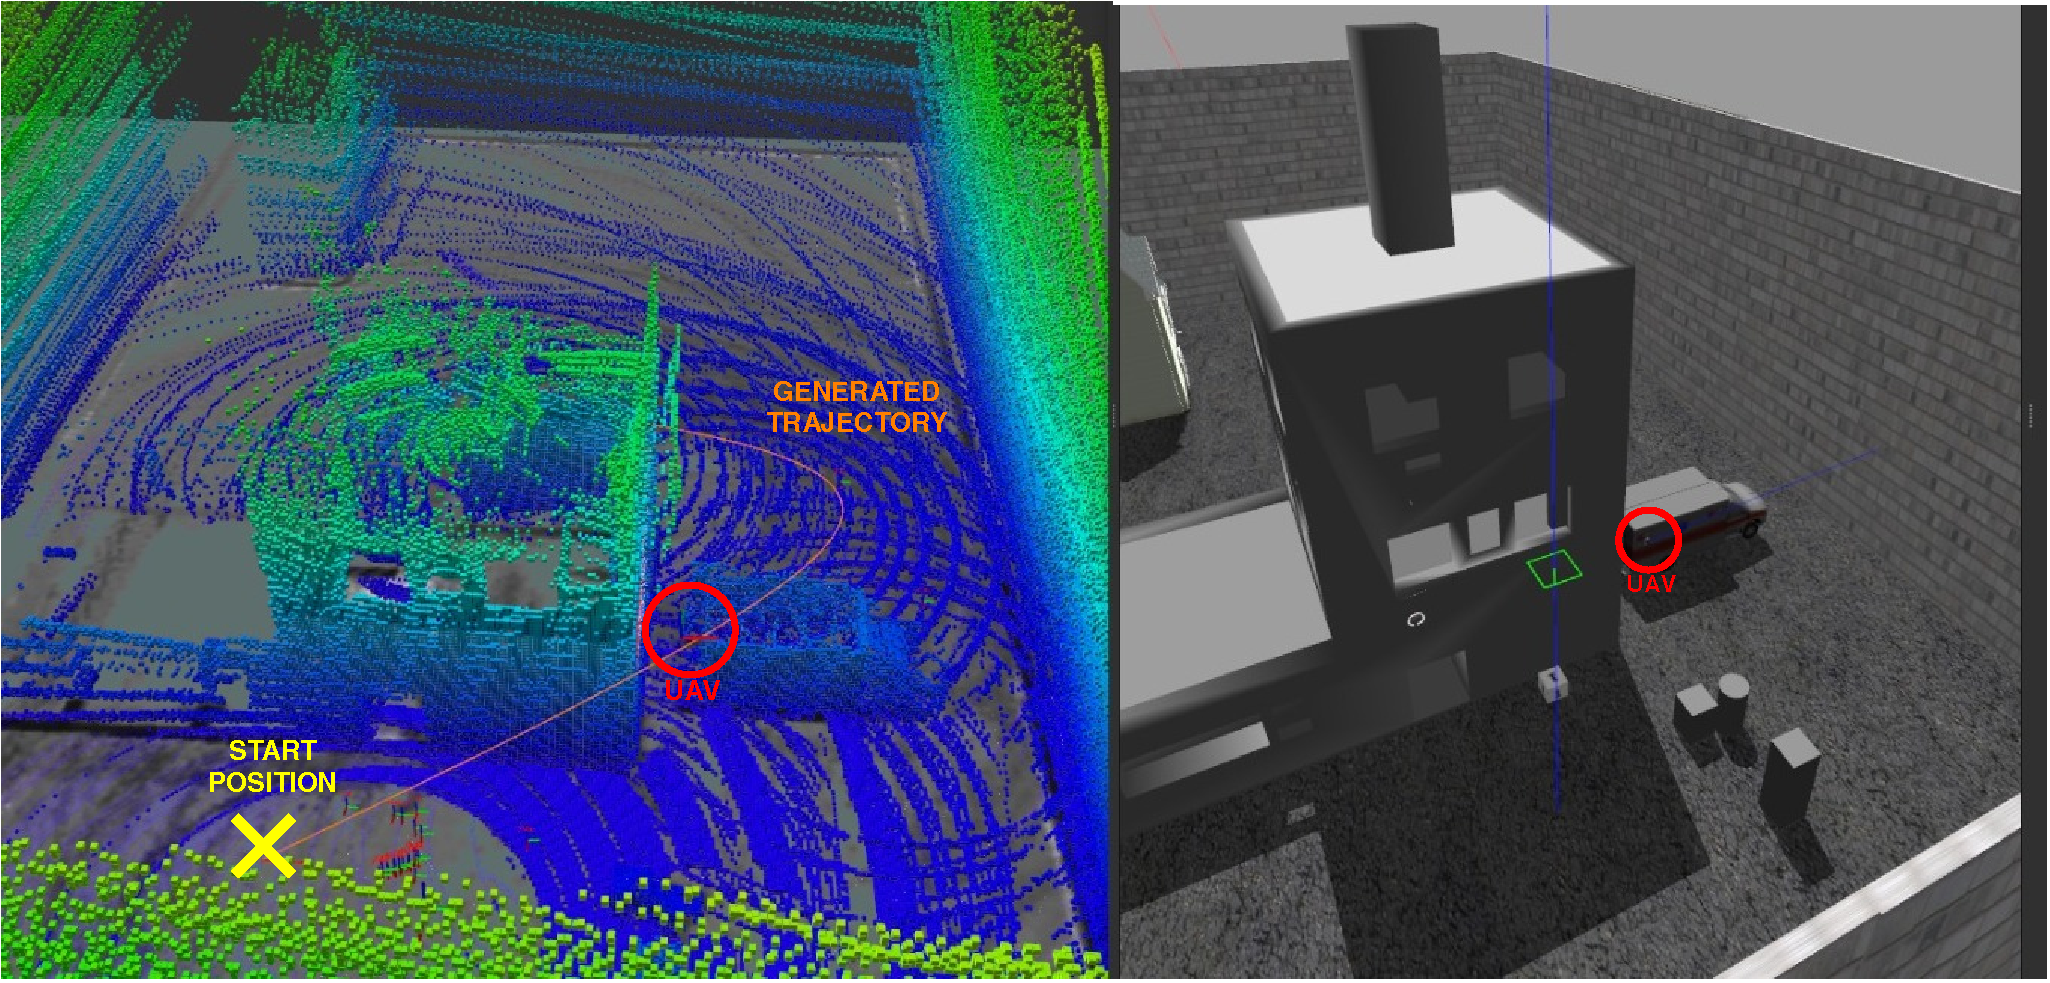
\includegraphics[height=3cm]{figures/rviz_gazebo}
	\end{figure}
		
\end{frame}

\begin{frame}
	\frametitle{Firefighting mission - real life scenario}
	\begin{columns}
		\begin{column}{0.5\textwidth}\centering
			\begin{center}
				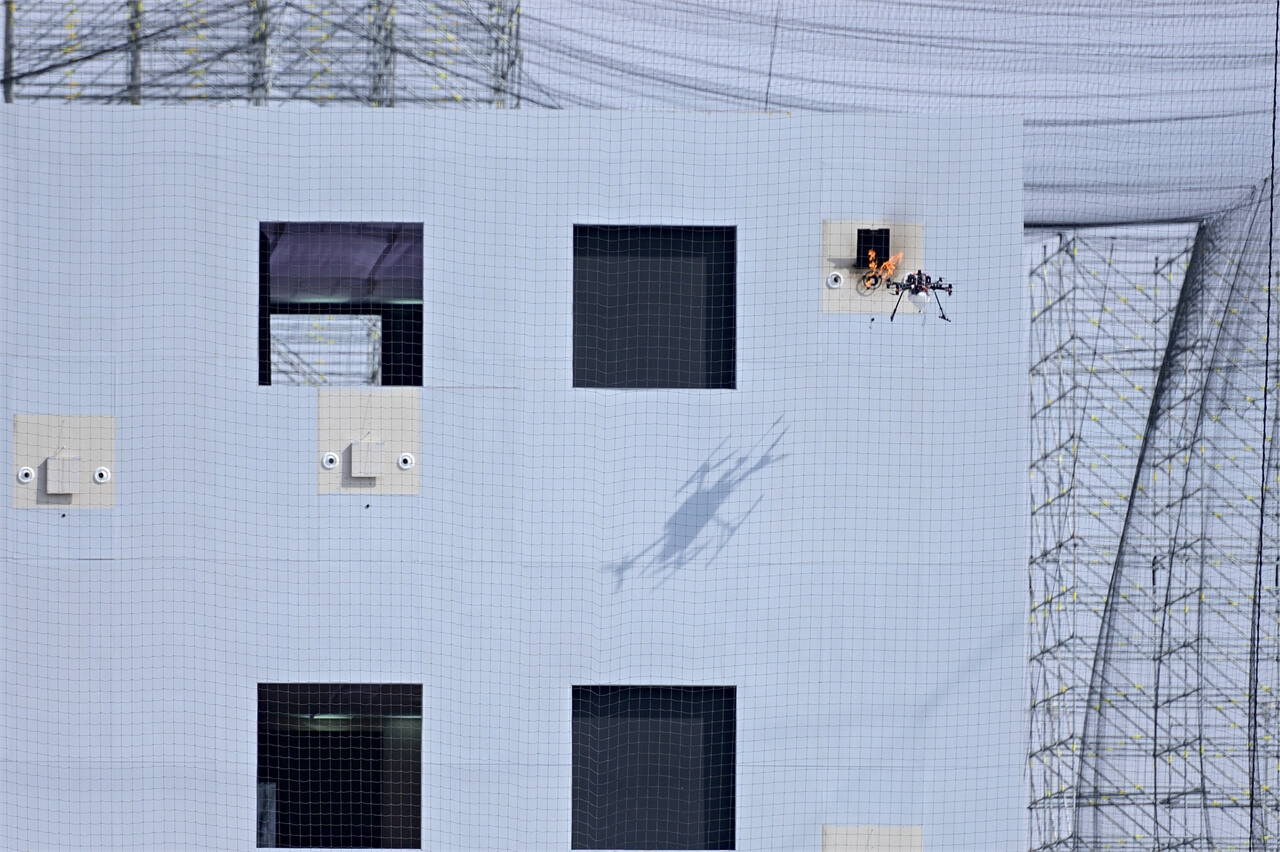
\includegraphics[width=1\textwidth]{figures/mbzirc_1}
				\label{fig:forest_uav}
			\end{center}
		\end{column}
		\begin{column}{0.5\textwidth}\centering
			\begin{center}
				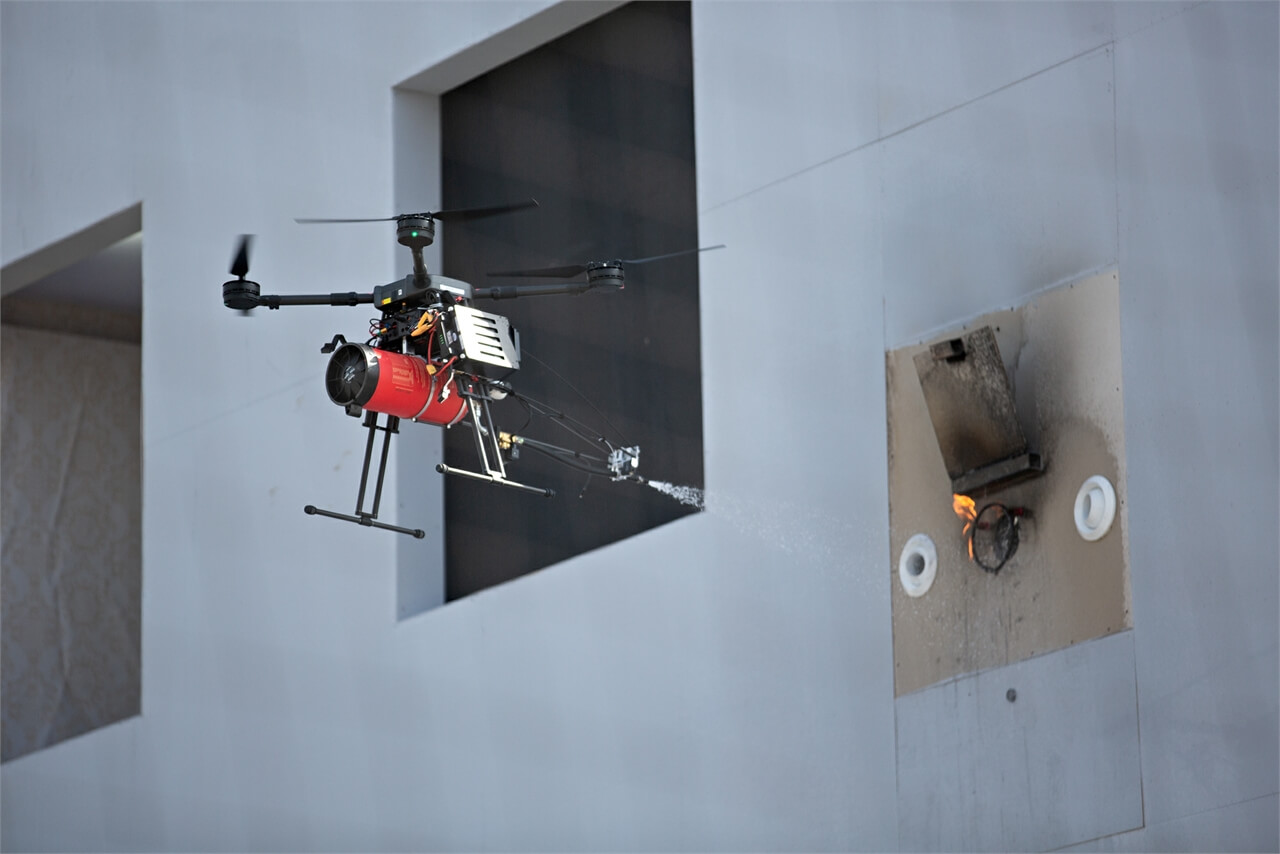
\includegraphics[width=1\textwidth]{figures/mbzirc_2}
				\label{fig:forest_uav}
			\end{center}
		\end{column}
	\end{columns}
	
\end{frame}
\section{Conclusion and future work}

\begin{frame}
	\frametitle{Conclusion and future work}
	\begin{columns}
		\begin{column}{0.6\textwidth}\centering
			
			\begin{itemize}
				\item[-] Brief overview of exploration strategies 
				\item[-] A modular approach to autonomous distributed multi-robot exploration and mapping\\
				\textbf{Future work:}  
				\item[-] Map decentralization using multi-robot system
				\item[-] Frontier detection and filtering problem in both 2D and 3D spaces 
				\item[-] Huge potential in fields like forestry, speleology, etc.
				\end{itemize} 
		\end{column}
	\begin{column}{0.5\textwidth}\centering
		\begin{center}
			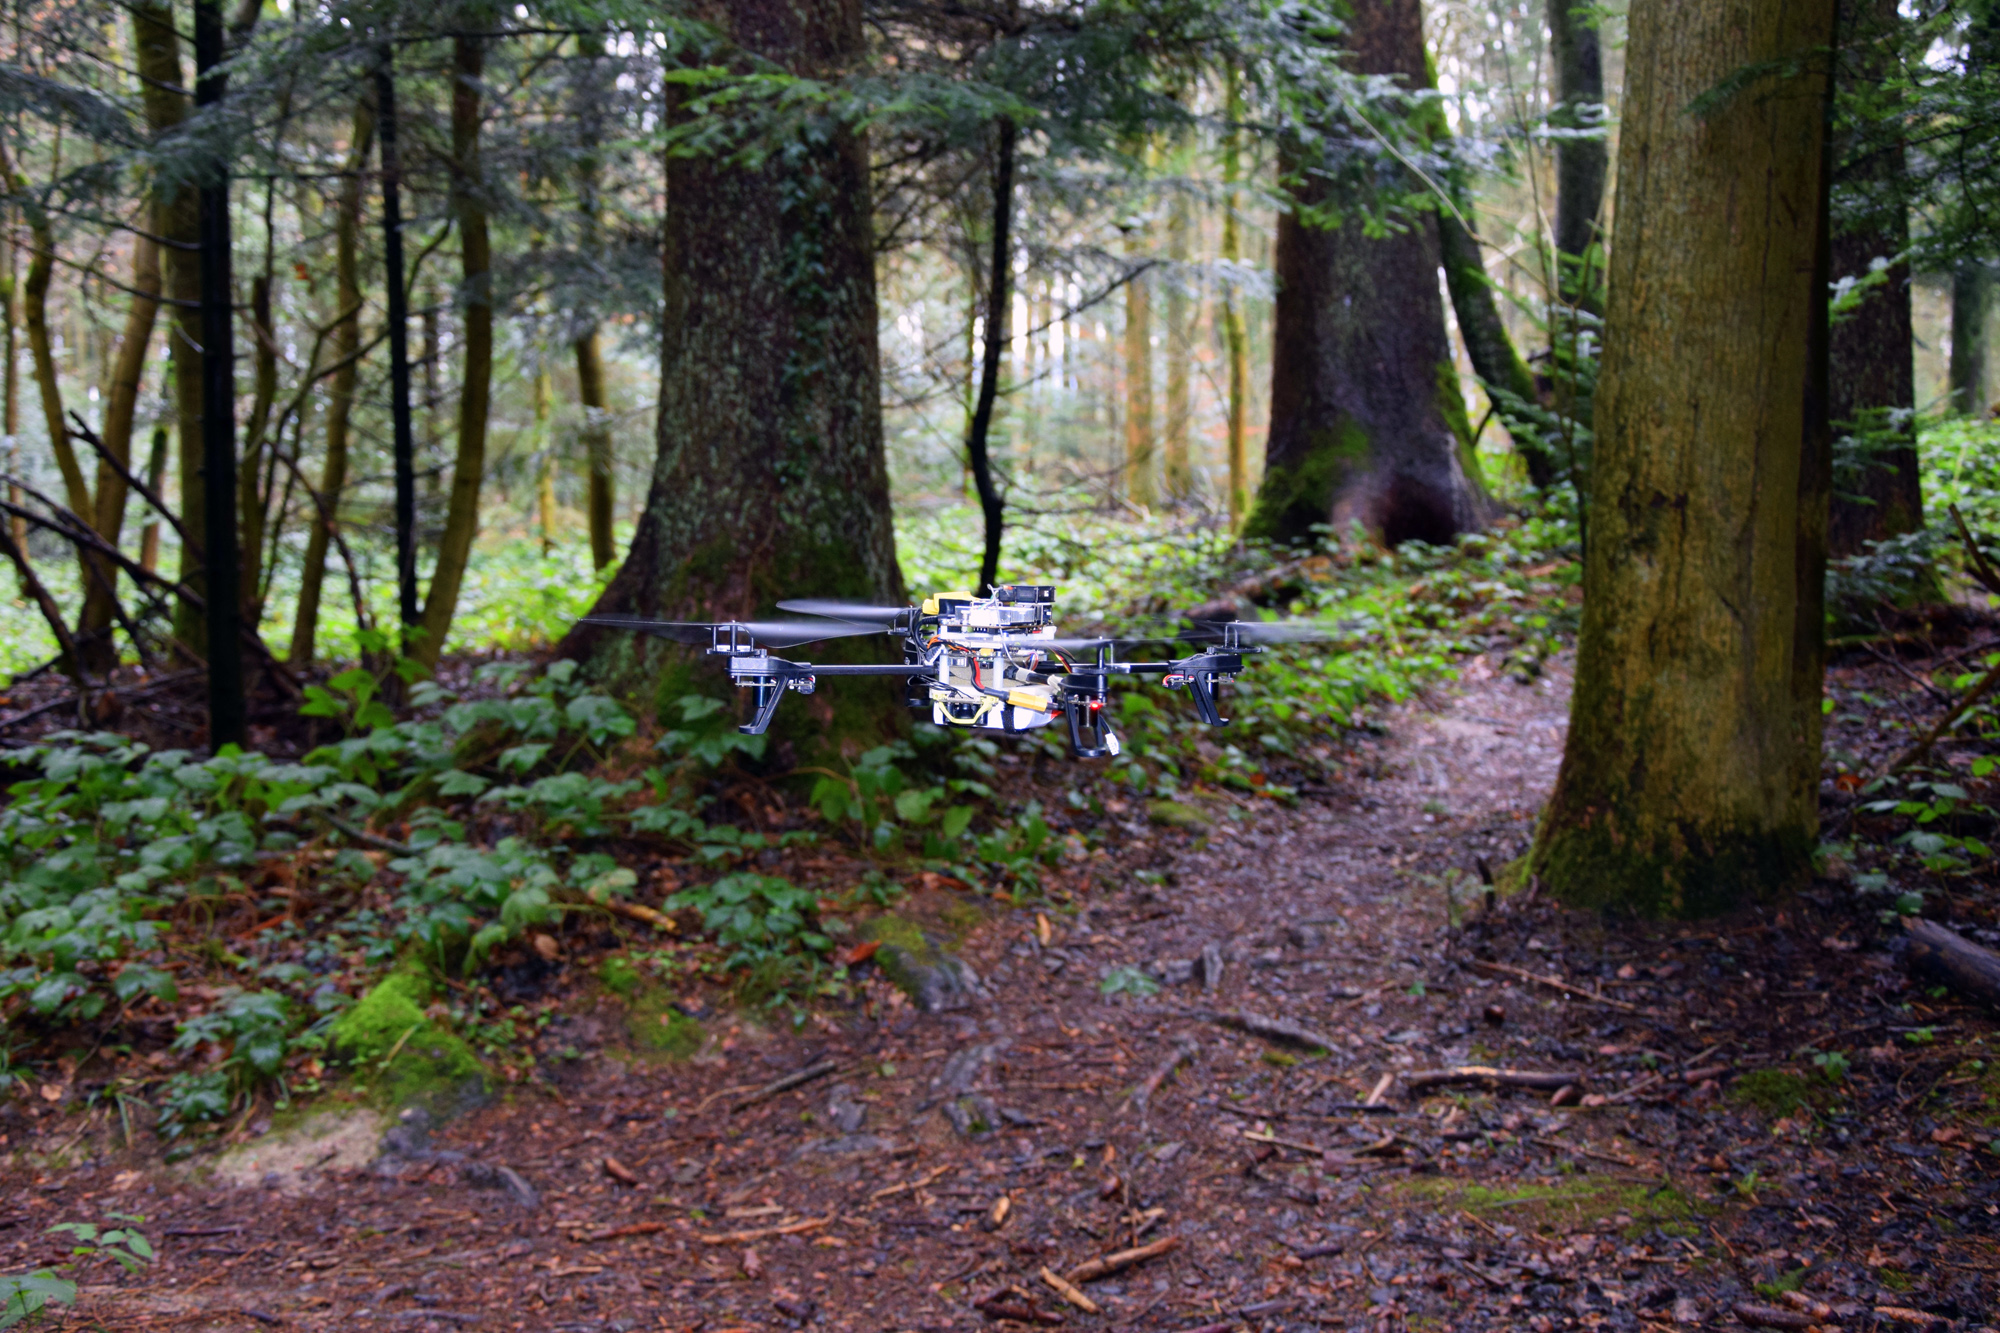
\includegraphics[height=3.5cm]{figures/forest-uav}
			\label{fig:forest_uav}
		\end{center}
%		\begin{center}
%		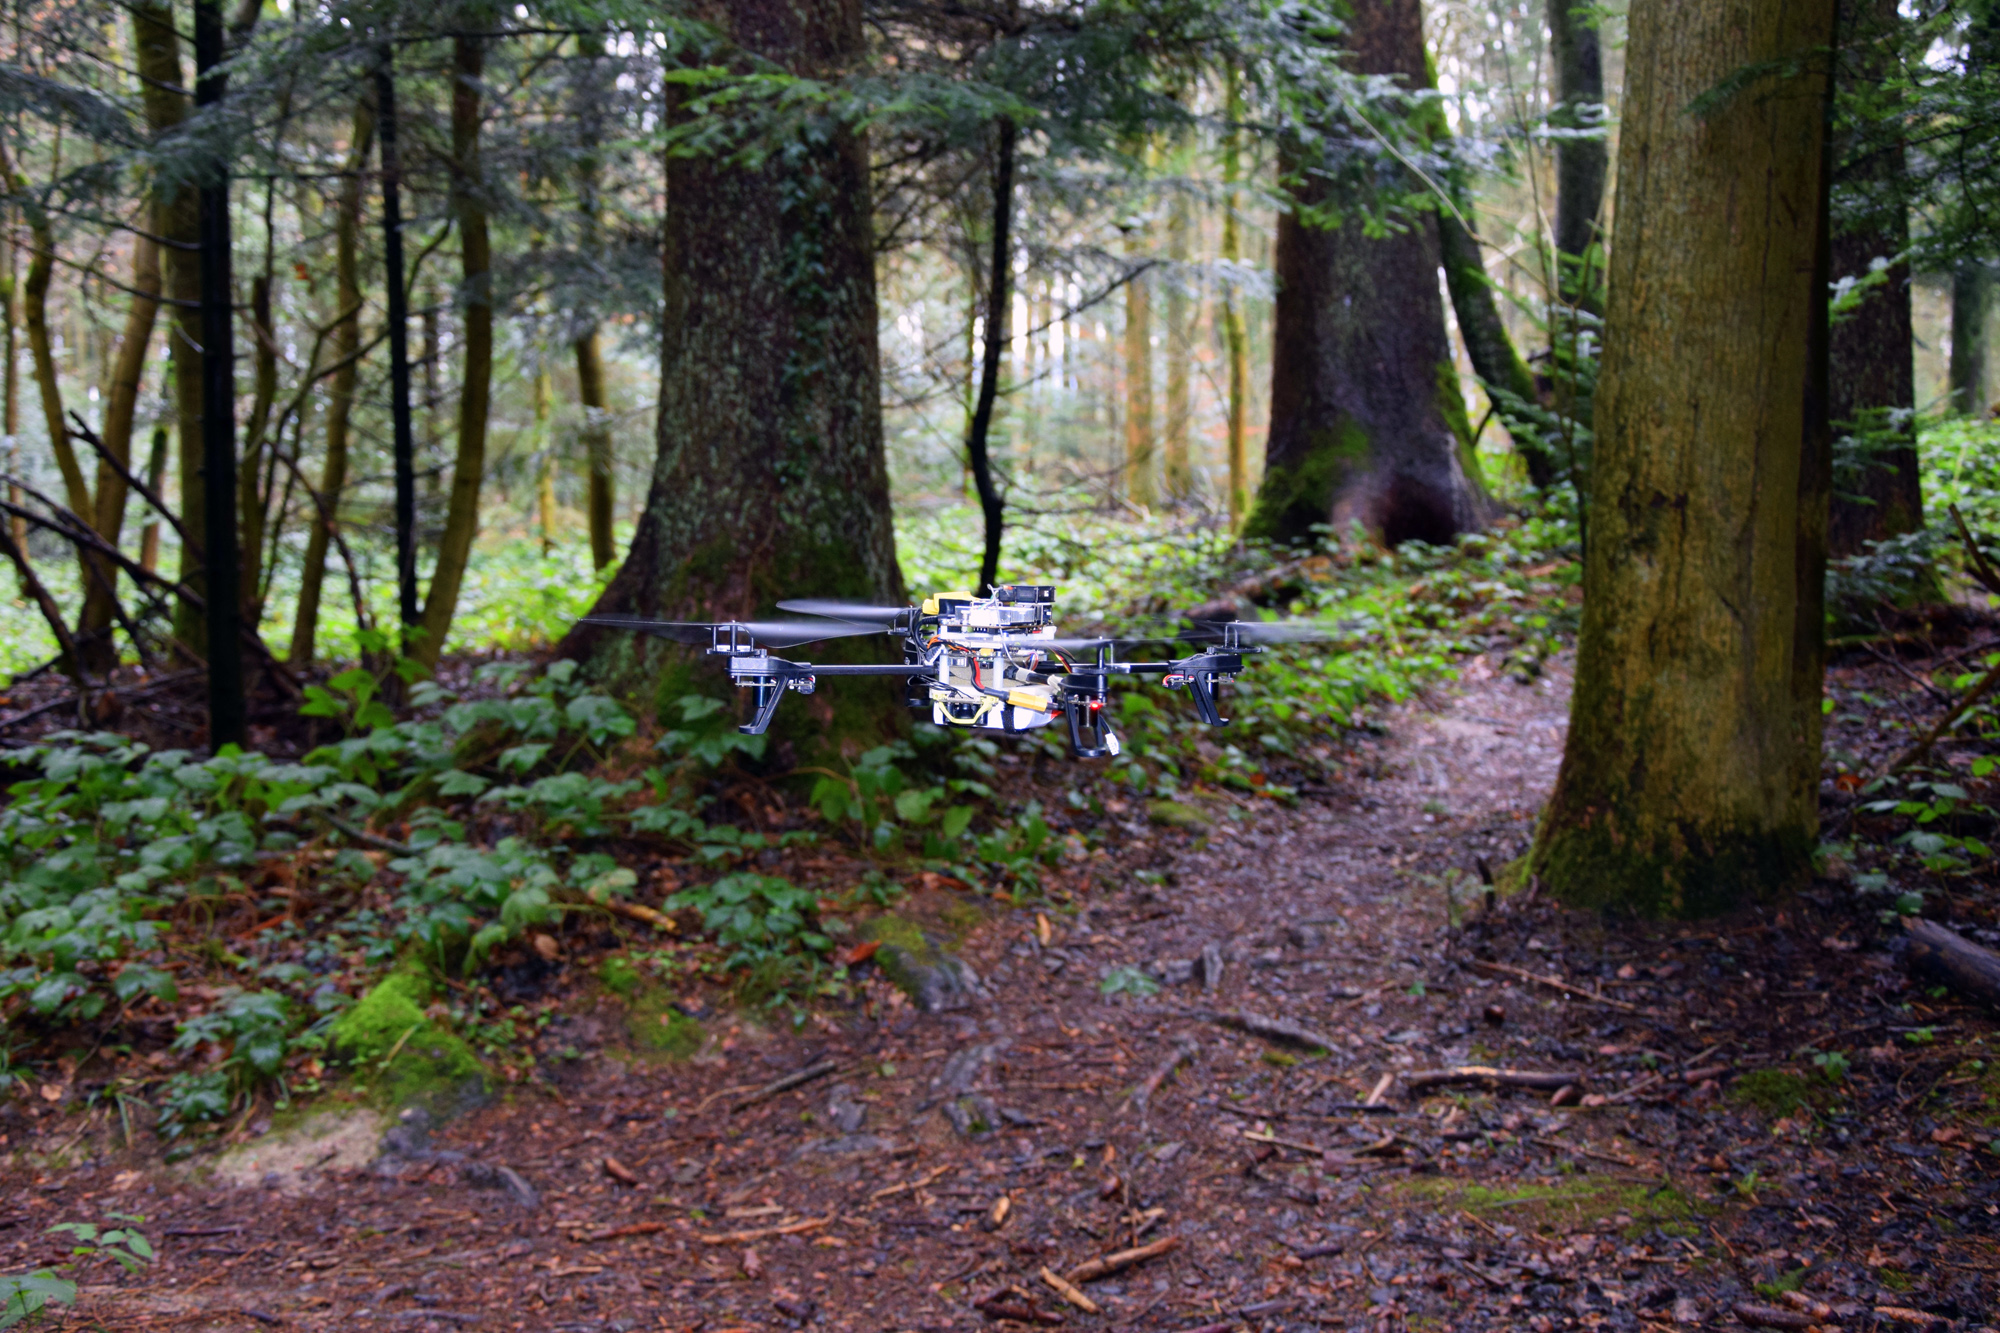
\includegraphics[height=3.5cm]{figures/forest-uav}
%		\label{fig:forest_uav}
%		\end{center}
		%			\vspace{0.1cm}
		%			\begin{itemize}
		%				\item Stiff position-controlled
		%				\item Payload: 10-300 kg
		%				\item High speed, high accuracy
		%			\end{itemize}
	\end{column}
\end{columns}
\end{frame}

%sadrzaj prezentacije
%\begin{frame}
%	\frametitle{Content}
%	\begin{itemize}
%		\item[1)] Introduction
%		\item[2)] Autonomous exploration
%		\item[3)] 2D exploration strategies
%		\item[5)] Conclusion and future work
%	\end{itemize}
%\end{frame}


\section*{Literatura}
\begin{frame}[allowframebreaks]{Literatura}
\printbibliography
\end{frame}

\end{document}